\chapter{Multiscale Geometric Analysis on the Sphere}
\minitoc 

\label{ch_mrs}

\vskip1cm

\index{wavelet}
\index{sphere}

\section{Introduction}

Many wavelet transforms on the sphere have been proposed in the past years.  Using the lifting scheme
 \citet{wave:sweldens95a} developed an orthogonal Haar wavelet 
 transform on any surface, which can be directly applied on the sphere.
 Its interest is however relatively limited because of the poor properties of the Haar function and the
 problems inherent to orthogonal transforms. 

More interestingly, many papers have presented 
 new continuous wavelet transforms \citep{wave:antoine99,wave:tenerio99,wave:cayon01,wave:holschneider96}.
 These works have been extended to directional wavelet transforms \citep{wave:antoine01,wave:hobson04}. 
 All these  continuous wavelet decompositions  are useful for data analysis, but cannot be used for restoration purposes because of the lack 
 of an inverse transform. 
\citet{freeden97} and \citet{freeden98} proposed the first redundant wavelet transform, based on the spherical harmonics transform, which presents an inverse transform.  
 \citet{starck:sta05_2}  proposed an invertible isotropic undecimated wavelet transform (UWT) on the sphere, also  based on 
spherical harmonics, which  has the same property as the starlet transform, i.e.\ the sum of the wavelet  scales reproduces the original image.
 A similar wavelet construction \citep{marinucci08,fay08a,fay08} used the so-called needlet filters.
 \citet{wiaux08} also proposed an algorithm which permits to reconstruct an image from its steerable wavelet transform.
Since reconstruction algorithms are available,  these new tools can be used for many applications
such as denoising, deconvolution, component separation \citep{starck:yassir05,bobin-gmca-cmb,delabrouille08} or inpainting \citep{inpainting:abrial06,starck:abrial08}.
\index{needlet filters}

Extensions to the sphere of 2D geometric multiscale decompositions such as the ridgelet 
transform and the curvelet transform were presented  in  
\citet{starck:sta05_2}.
  % It has been shown that such constructions are very useful for the detection of cosmic strings \citep{starck:sta03_1,starck:jin05,hammond08}.

The goal of this chapter is to overview these multiscale transforms on the sphere. Section~\ref{mrs_pixel} overviews the HEALPix pixelization scheme and the spherical harmonics transform. Section~\ref{mrs_haar} shows how a fast orthogonal Haar wavelet transform on the sphere can be built using HEALPix. In Section~\ref{sect_wts}, we present an isotropic wavelet transform on the sphere which has similar properties as the starlet transform and therefore should
be very useful for data denoising and deconvolution. This algorithm is directly derived from the FFT-based wavelet transform proposed in \citet{starck:sta94_3} for aperture synthesis image restoration (see Section~\ref{sec_fft}), and is relatively close to the \citet{freeden98} method, except that it features the same straightforward reconstruction as does the starlet transform algorithm (i.e.\ the sum of the scales reproduces the original data). This wavelet transform can also be easily extended to a pyramidal wavelet transform, allowing us to reduce the redundancy, a possibility which may be very important for larger data sets. In Section~\ref{sect_cur}, we show how this new pyramidal transform can be used to derive a curvelet transform on the sphere. Section~\ref{sect_exp} describes how these new transforms can be used for denoising, component separation and inpainting. 

Sections~\ref{section:bedros} and \ref{section:cmb} present how these new tools can help us to analyze data in two real applications, in physics and in cosmology. Finally, guided numerical experiments together with a toolbox dedicated to multiscale transforms on the sphere (MR/S) are described.
 
\section{Data on the Sphere}
\label{mrs_pixel}

Various pixelization schemes for data on the sphere exist in the literature. These include the Equidistant Coordinate Partition (ECP), the Icosahedron method  \citep{tegmark:icos1}, the Quad Cube \citep{white92}, IGLOO \citep{igloo}, HEALPix \citep{pixel:healpix}, Hierarchical Triangular Mesh (HTM) \citep{kunszt01} or Gauss-Legendre Sky Pixelization (GLESP) \citep{pixel:glesp}. Important properties to decide which one is the best for a given application include the number of pixels and their size, fast computation of the spherical harmonics transform, equal surface area for all pixels, pixel shape regularity, separability of variables with respect to latitude and longitude, availability of efficient software libraries including parallel implementation, etc. Each of these properties has advantages and drawbacks. In this chapter, we use the HEALPix representation which has several useful properties. 

\newpage
\subsection{HEALPix}
\index{HEALPix}
\label{healpix}

\begin{figure}[htb]
\centering
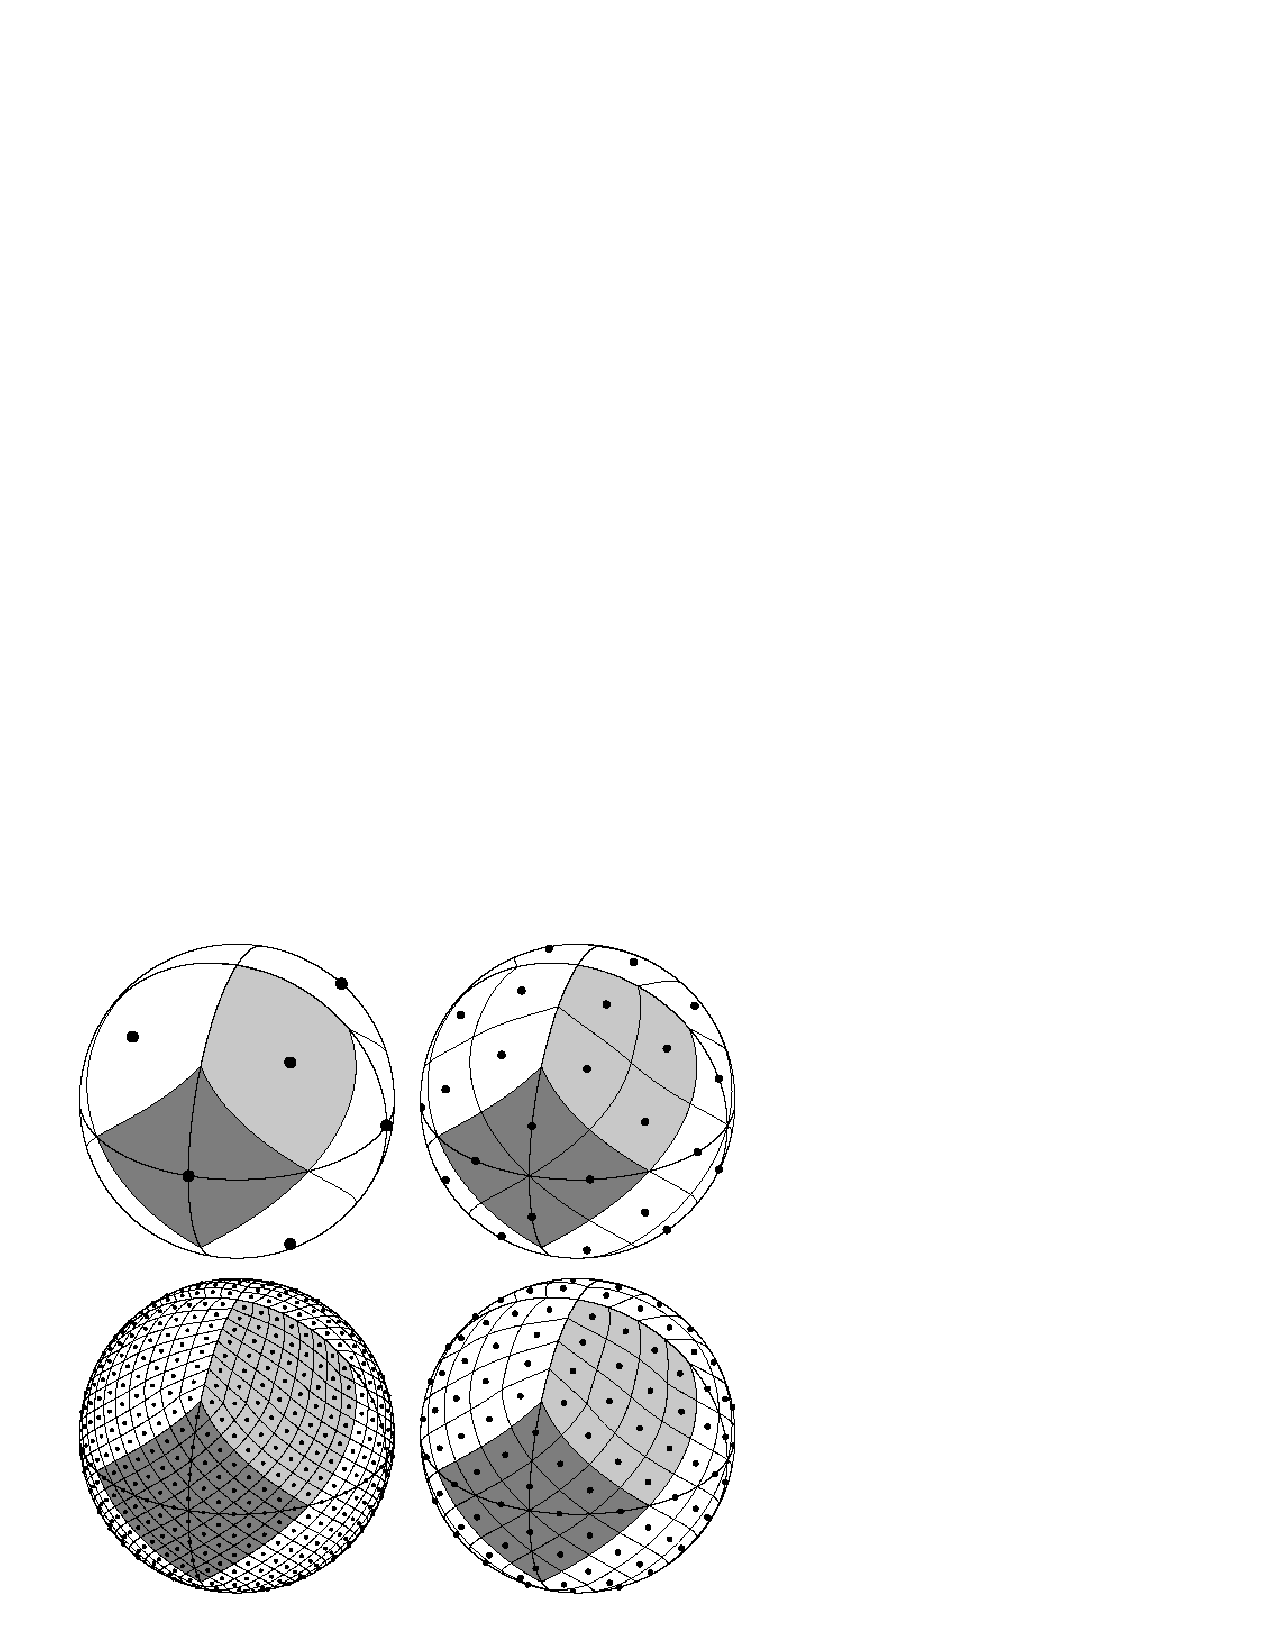
\includegraphics[width=8cm]{pixelhealpix.pdf}
\caption{The HEALPix sampling grid for four different resolutions.}
\label{pixelhealpix}
\end{figure}

The HEALPix representation (Hierarchical Equal Area isoLatitude Pixelization of a sphere) \citep{pixel:healpix}\footnote{http://healpix.jpl.nasa.gov.} is a curvilinear hierarchical partition of the sphere into quadrilateral pixels of exactly equal area but with varying shape. The base resolution divides the sphere into 12 quadrilateral faces of equal area placed on three rings around the poles and equator. Each face is subsequently divided into $N_{\mathrm{side}}^{2}$ pixels following a quadrilateral multiscale  tree structure (see Fig.~\ref{pixelhealpix}). The pixel centers are located on iso-latitude rings, and pixels from the same ring are equispaced in azimuth. This is critical for computational speed of all operations involving the evaluation of the spherical harmonics coefficients, including standard operations such as convolution, power spectrum estimation, and so on.  
HEALPix is a standard pixelization scheme in astronomy.
 
% \begin{figure*}
%\centering
%\includegraphics[height = 2.8 in]{pixelbasecyl.pdf}
%\caption[Projection cylindrique de diff\'erentes pix\'elisations possibles.]{Projection cylindrique de diff\'erentes pix\'elisations possibles pour diff\'erents $N_\theta$ et $N_\vartheta$. La grille HEALPix utilise $N_\theta=3$ et $N_\vartheta =4$}
%\label{pixcyl}
%\end{figure*}

% La pix\'elisation s'effectue en d\'ecoupant la surface form\'ee suivant la projection cylindrique en $N_\theta$ et $N_\vartheta$ parties suivant respectivement la latitude et la longitude, 
% selon les figures \ref{pixcyl} et \ref{pixsph}. La s\'eparation entre les pixels pres du pôle et ceux pres de l'\'equateur est choisie de telle façon que tous les pixels aient  la même surface.
% Du fait de ce choix de pix\'elisation de base, les frontieres de chaque pixel sont assez simples. Elles sont de la forme $cos{\theta} = a + b * \vartheta $ dans la zone \'equatoriale et de la forme $ cos{\theta} = a + b / (\vartheta)^2 $ ailleurs.

% Pour leur implantation, ils ont choisi $N_\theta = 3$ et $N_\vartheta = 4$, si bien que la pix\'elisation de base comporte 4 pixels autour de chaque pôle et 4 pixels le long de l'\'equateur.

% \begin{figure*}
% \centering
% \includegraphics[height = 2.8 in]{pixelbasesph.pdf}
% \caption[Projection orthographique de diff\'erentes pix\'elisations possibles.]{Projection orthographique de diff\'erentes pix\'elisations possibles pour diff\'erents $N_\theta$ et $N_\vartheta$. }
% \label{pixsph}
% \end{figure*}
 

\subsection{Spherical Harmonics}
\index{spherical harmonics}

The equivalent of the Fourier transform on the sphere is the spherical harmonics transform. From this analogy, in the sequel, the $\hat{ }$ notation that was used for Fourier transform in previous chapters will be used to denote the spherical harmonics coefficients of a function. 
Any function $f(\theta,\vartheta) \in L_2(S^2)$ on the sphere $S^2$ in $\RR^3$ can be decomposed into spherical harmonics:
\begin{eqnarray}
\label{decomp_alm}
f(\theta,\vartheta)=\sum_{l=0}^{+\infty}\sum_{m=-l}^{l} \hat{f}_{lm}Y_{lm}(\theta,\vartheta) ,
\end{eqnarray}
where  $Y_{lm}$ are the spherical harmonics defined by:
\begin{eqnarray}
\label{def_ylm}
Y_{lm}(\theta,\vartheta)=\sqrt{\frac{2l+1}{4\pi}\frac{(l- \abs{m} )!}{(l+ \abs{m} )!}} P_{lm}(\cos\vartheta)e^{im\theta},
\end{eqnarray}

$P_{lm}$ are the  associated Legendre functions (or polynomials) defined by the following differential equation:
\begin{eqnarray}
\label{def_poly_legendre}
\frac{d}{dt} \left[     (1-t^2)   \frac{d}{dt} P_{lm}  \right]   + \Big( l(l+1) - \frac{m^2}{1-t^2}\Big) P_{lm} = 0  .
\end{eqnarray}

These functions are related to the Legendre polynomials $P_{l}$ by 
\begin{eqnarray}
P_{lm}(t)  = (-1)^m (1-t^2)^{m/2}\frac{d^m}{dt^m}P_l(t) ,
\label{def_poly_leg}
\end{eqnarray}
where  $P_l$  is:
\begin{eqnarray}
P_{l}(t)  =\frac{1}{2^l l!}  \frac{d^l}{dt^l} (t^2-1)^l .
\label{def_pl}
\end{eqnarray}

Furthermore, an important property of the Legendre polynomials is that they are orthogonal:  
\begin{eqnarray}
\label{ortho_harm_sph}
\sum_{l\in\mathbb{N}} \sum_{|m|\leqslant l} Y^*_{lm}({\boldsymbol \omega}') \ Y_{lm}({\boldsymbol \omega}) = \delta({\boldsymbol \omega}' - {\boldsymbol \omega}) .
\end{eqnarray}
with ${\boldsymbol \omega} = (\theta,\vartheta)$ et ${\boldsymbol \omega}' = (\theta',\vartheta')$


%  On peut ainsi souhaiter que la transform\'ee en harmoniques sph\'eriques possede un algorithme rapide. 
% On peut \'egalement vouloir qu'elle soit inversible pour des images à bande limit\'ee.
% Pour le premier point, il est indispensable que les points soient \'equir\'epartis
% sur les m\'eridiens et les paralleles. Pour le deuxieme point, il suffit que
% l'\'echantillonage en $\vartheta $ soit suffisant et que les points d'\'echantillonage
% en latitude  $\theta $ appartiennent, soit aux z\'eros du polynôme de Legendre ou qu'ils soient \'equir\'epartis.


In this chapter, many multiscale decompositions will be built 
based on the spherical harmonics and/or the HEALPix representation.

\section{Orthogonal Haar Wavelets on the Sphere}
\label{mrs_haar}
\index{wavelet!Haar on sphere}
\index{sphere!Haar}

The Haar wavelet transform on the sphere  \citep{wave:sweldens95a} 
at each resolution $j$ and pixel $\bk=(k_x,k_y)$ on the sphere is based on a scaling function  $\phi_{j,\bk}$ ($\phi_{j,\bk}(\bx) = \phi\parenth{2^{-j}(\bx-\bk)}$, where $\bx$ is the vector of Cartesian coordinates on the sphere, and $\phi$ is the Haar scaling function) 
and three Haar wavelet functions $\psi^{d}_{j,\bk}$ (see Section~\ref{sec_haar})
with  $d \in\{1,2,3\}$. It uses the idea that a given pixel on the sphere at a given resolution $j$  in the HEALPix representation
is directly related to four pixels at the next resolution $j-1$.  
% For Healpix  pixelisation, resolution of the map is related 
% to the  $N_{side}$ parameter, 
% which corresponds to the square root of number of pixels in each face.
% $ N_{side} = 2^{j-1}$.  At a given resolution  $j$ we have $n_j=12 \times 4^{j-1}$ pixels with a surface size $\mu_j$. 

% Noting, $\bk_0$, the pixelThe scaling function $\phi$ and three wavelet functions $\psi$ are defined by:
% \begin{eqnarray}
% \label{def_whaar1}
% \phi_{j,\bk}(\bx) & = & \left\{  \begin{array}{ll}
% 1 & \textrm{si $t \in S_{j,\bk}$ }\\
% 0 & \textrm{sinon}
%    \end{array} \right.  \nonumber \\
% \psi_{1,j+1,\bk} & = & \frac{\phi_{j,\bk_0} +\phi_{j,\bk_2}-\phi_{j,\bk_1}-\phi_{j,\bk_3} } {4}   \nonumber \\
% \psi_{2,j+1,\bk} & = & \frac{\phi_{j,\bk_0} +\phi_{j,\bk_1}-\phi_{j,\bk_2}-\phi_{j,\bk_3} }{4}  \nonumber \\
% \psi_{3,j+1,\bk} & = & \frac{\phi_{j,\bk_0} +\phi_{j,\bk_3}-\phi_{j,\bk_1}-\phi_{j,\bk_2} }{4}
% \end{eqnarray}

% \begin{figure}[htb]
%\centering
%\includegraphics[width=10cm]{fig_haar_decomp.pdf}
%\label{fig_haar_decomp}
%\caption{On resolution to next using Haar.}
%\end{figure}

% \begin{figure*}
% \vbox{
% \centerline{
% \hbox{
% \includegraphics[angle=180,width=7cm]{haar0.pdf}
% \includegraphics[angle=180,width=7cm]{haar1.pdf}
% }}\centerline{
% \hbox{
% \includegraphics[angle=180,width=7cm]{haar2.pdf}
% \includegraphics[angle=180,width=7cm]{haar3.pdf}
% }}
% \centerline{
% \hbox{
% \includegraphics[angle=180,width=7cm]{haar4.pdf}
% \includegraphics[angle=180,width=7cm]{haar5.pdf}
% }}
% }
% \label{fig_haar_decomp2}
% \caption{Haar wavelet  coefficents.}
% \end{figure*}

Denoting $\bk_0,\bk_1,\bk_2,\bk_3$  the four pixels at scale $j$, hierarchically related to 
the pixel $\bk$ at scale $j+1$,  scaling coefficients  $c_{j+1,\bk}$ at scale $j+1$ are derived from 
  those at scale $j$ by:
\begin{eqnarray}
\label{def_haar1}
c_{j+1}[\bk] &=& \frac{1}{4} \sum_{d=0}^3 c_{j} [\bk_d],
\end{eqnarray}
and wavelet coefficients at scale $j+1$ from coefficients at scale  $j$ by:
\begin{eqnarray}
\label{def_haar2}
w^{1}_{j+1} [\bk] &=& \frac{1}{4} (c_{j}[\bk_0]+c_{j} [\bk_2]   -  c_{j} [\bk_1]-c_{j}[\bk_3])  \nonumber  \\
w^{2}_{j+1} [\bk] &=&\frac{1}{4}  (c_{j}[\bk_0]+c_{j} [\bk_1]   -  c_{j}[\bk_2]-c_{j}[\bk_3])  \nonumber  \\
w^{3}_{j+1} [\bk] &=&\frac{1}{4}  (c_{j}[\bk_0]+c_{j} [\bk_3]   -  c_{j} [\bk_1]-c_{j}[\bk_2]) .
\end{eqnarray}

% Fig. \ref{fig_haar_decomp} shows the calculation scheme of haar coefficients, from one resolution to the next. 
% Haar wavelet coefficients for the astronomical WMAP data set are shown in Fig. \ref{fig_haar_decomp2}.

The Haar wavelet transform on the sphere is orthogonal and its reconstruction is exact. The inverse transformation is obtained by:
 \begin{eqnarray}
\label{def_recons_haar}
c_0[\bx] = \sum_{\bk}  c_{J}[\bk]  \phi_{J,\bk}(\bx) + \sum_{j=1}^{J} \sum_{d=1}^3 \sum_{\bk} w^{d}_{j}[\bk]  \psi^d_{j}(\bx) .
\end{eqnarray}

This transform is very fast but its interest is relatively limited. Indeed, it is not rotation invariant, and more importantly the Haar wavelet shape is not well adapted for most applications, because of the non-regular shape of the wavelet function.


% ===============================================

\section{Continuous Wavelets on the Sphere}

\subsection{Stereoscopic Projection}
\label{chap_mex_hat}

\index{wavelet!axisymmetrical wavelets}
\index{wavelet!stereoscopic projection}

\begin{figure}[htb]
\centering
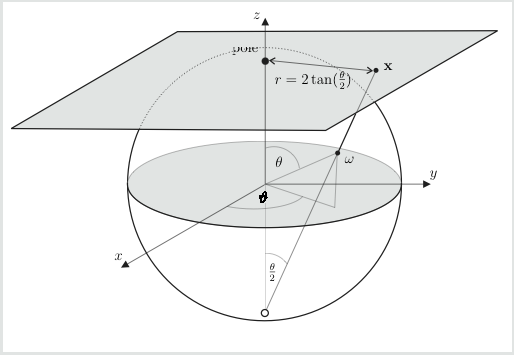
\includegraphics[width=10cm]{proj_stereo_inverse.pdf}
\caption{Inverse stereographic projections  of a  radial  function  from plane  to the  sphere.}
\label{figprojstereo_direct}
\end{figure}

In order to have more choice to design the wavelet function, we may want to use wavelets defined for regular 2D images to the sphere.
This is possible by using inverse stereographic projections of radial wavelet functions such the Mexican hat \citep{wave:cayon01}.
Defining the stereographic projection operator, $\bR: {\bf t}  \mapsto \ {\boldsymbol \omega} $, with $  {\boldsymbol \omega}  = (\theta(r),\vartheta) $, $\theta(r) = 2 \arctan(r/2)$,
the  radial wavelets $\psi_{\mathrm{plane}}$ can be projected on the sphere by a unique rotation,   ${\boldsymbol \omega}_0 =(\theta_0,\vartheta_0)$, respectively around the two axes   $O_y$ and $O_z$.  
Fig.~\ref{figprojstereo_direct} shows the projection of radial functions from the plane to the sphere. 
 
The convolution on the sphere between a radial wavelet function $\psi(\theta)$ and a function $f({\boldsymbol \omega})$ is:
 \begin{eqnarray}
\label{convol_sph}
(\psi \ast f)(\theta,\vartheta)= \int_{S^2} \psi_{\mathrm{plane}}^* (\bR^{-1}  {\boldsymbol \omega}) f({\boldsymbol \omega}) d{\boldsymbol \omega} .
\end{eqnarray}

Such wavelets are axisymmetric by construction. This property can be used to derive fast transformation algorithms using spherical harmonics.
Indeed spherical harmonics coefficients $\hat{\psi}[l,m]$ of the wavelet function $\psi$ on the sphere are equal to zero when  $m \neq 0$, and by the Funk-Hecke theorem, the convolution can be written using spherical harmonics by:
\begin{eqnarray}
\label{convol_sph_harm}
(\psi \ast f)(\theta,\vartheta)  =  \sum_{l=0}^{\infty} \sum_{m=-l}^{l} \sqrt{\frac{2l+1}{4\pi} }\hat{f}[l,m] \hat{ \psi}[l,0] Y_{lm}(\theta,\vartheta) ~.
\end{eqnarray}
where $\hat{f}[l,m]$ are the spherical harmonics coefficients of the function $f$, i.e. $f = \sum_{l=0}^{\infty}\sum_{m=-l}^{l}  \hat{f}[l,m] Y_{lm}$ and similary for $\hat{\psi}$.

Classical wavelet dilations can also be derived on the sphere using the dilation operator $\mathscr{D}_a$ by a factor $a > 0$ \citep{wiaux07}:
\begin{eqnarray}
\label{proj_stereo}
\mathscr{D}_a(f)({\boldsymbol \omega}) = \chi_a^{1/2} (a,\theta)  f(D^{-1}_a {\boldsymbol \omega}) ,
\end{eqnarray}
where $D_a(\theta,\vartheta)=(\theta_a(\theta),\vartheta)$ with the linear relation $\tan\theta_a(\theta)/2=a\tan\theta/2$, and $D_a$ is the dilation operator that maps a sphere without its South pole on itself. $ \chi_a^{1/2}(a,\theta)$ is a norm preservation term (i.e. $\mathscr{D}_a$ is unitary):
\begin{eqnarray}
\label{def_lambda}
\chi_a^{1/2}(a,\theta) = a^{-1}[1+\tan^2(\theta/2)]/[1+a^{-2}\tan^2(\theta/2)] ~.
\end{eqnarray}

% \begin{figure*}
% \centering
% \includegraphics[width=9cm]{proj_stereo.pdf}
% \caption{Projection st\'er\'eographique inverse sur la sphere.}
% \label{figprojstereo}
% \end{figure*}

\subsection{Mexican Hat Wavelet} 

\index{wavelet!Mexican hat on sphere}
\index{sphere!Mexican hat}
\index{Mexican hat!on sphere}

\begin{figure}[htb]
\vbox{
\centerline{
\hbox{
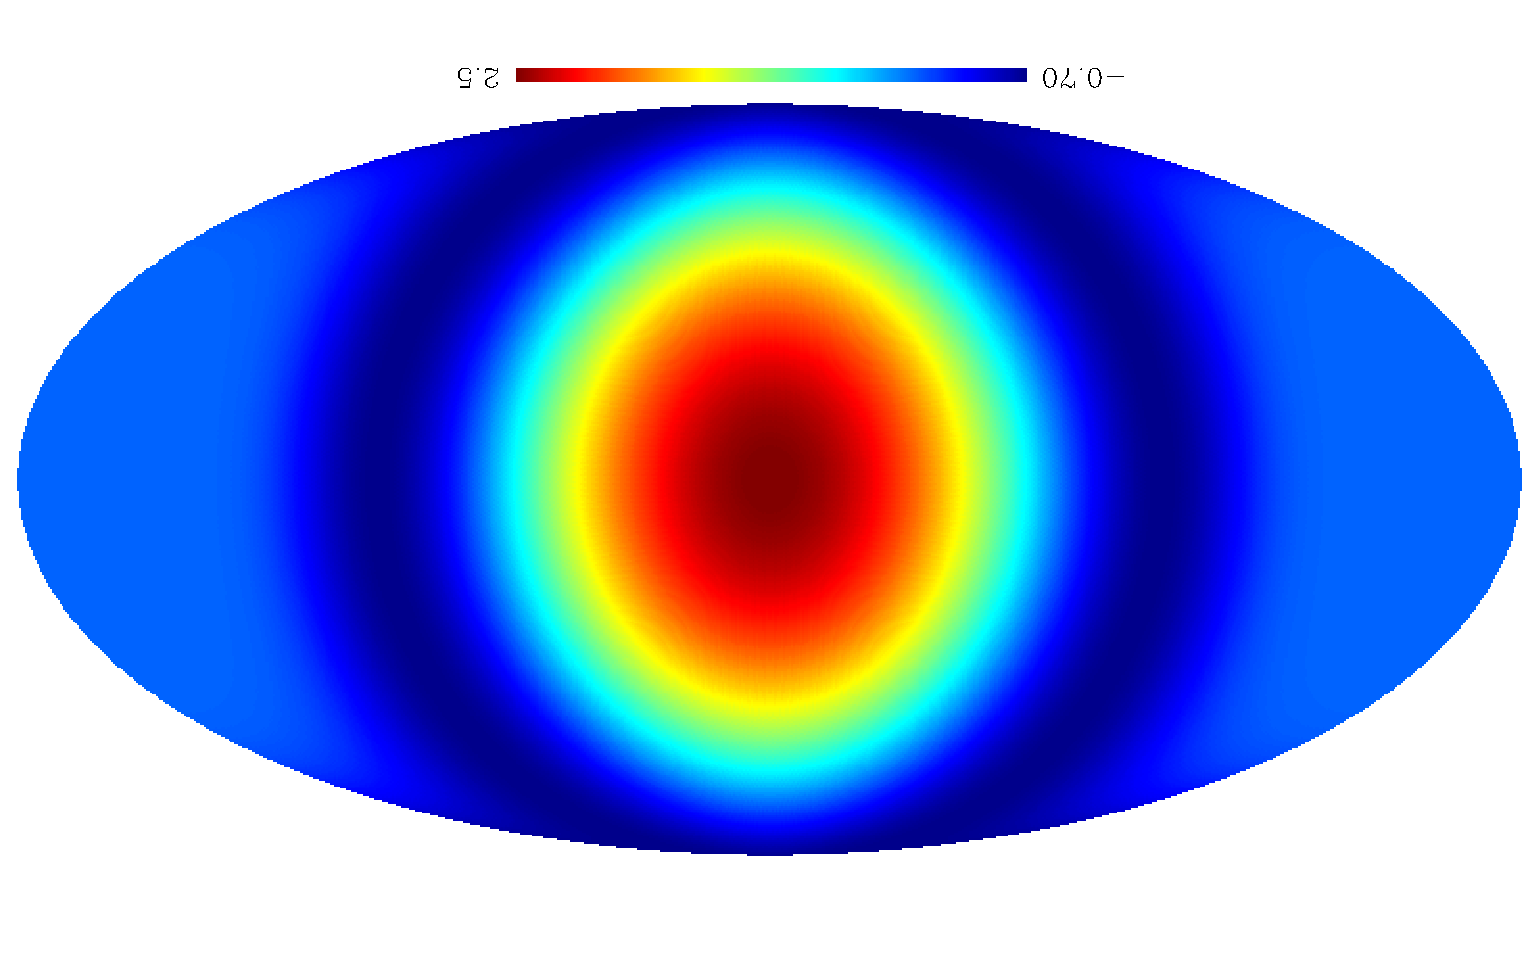
\includegraphics[angle=180,width=6.5cm]{wav_mex_hat_0.pdf}
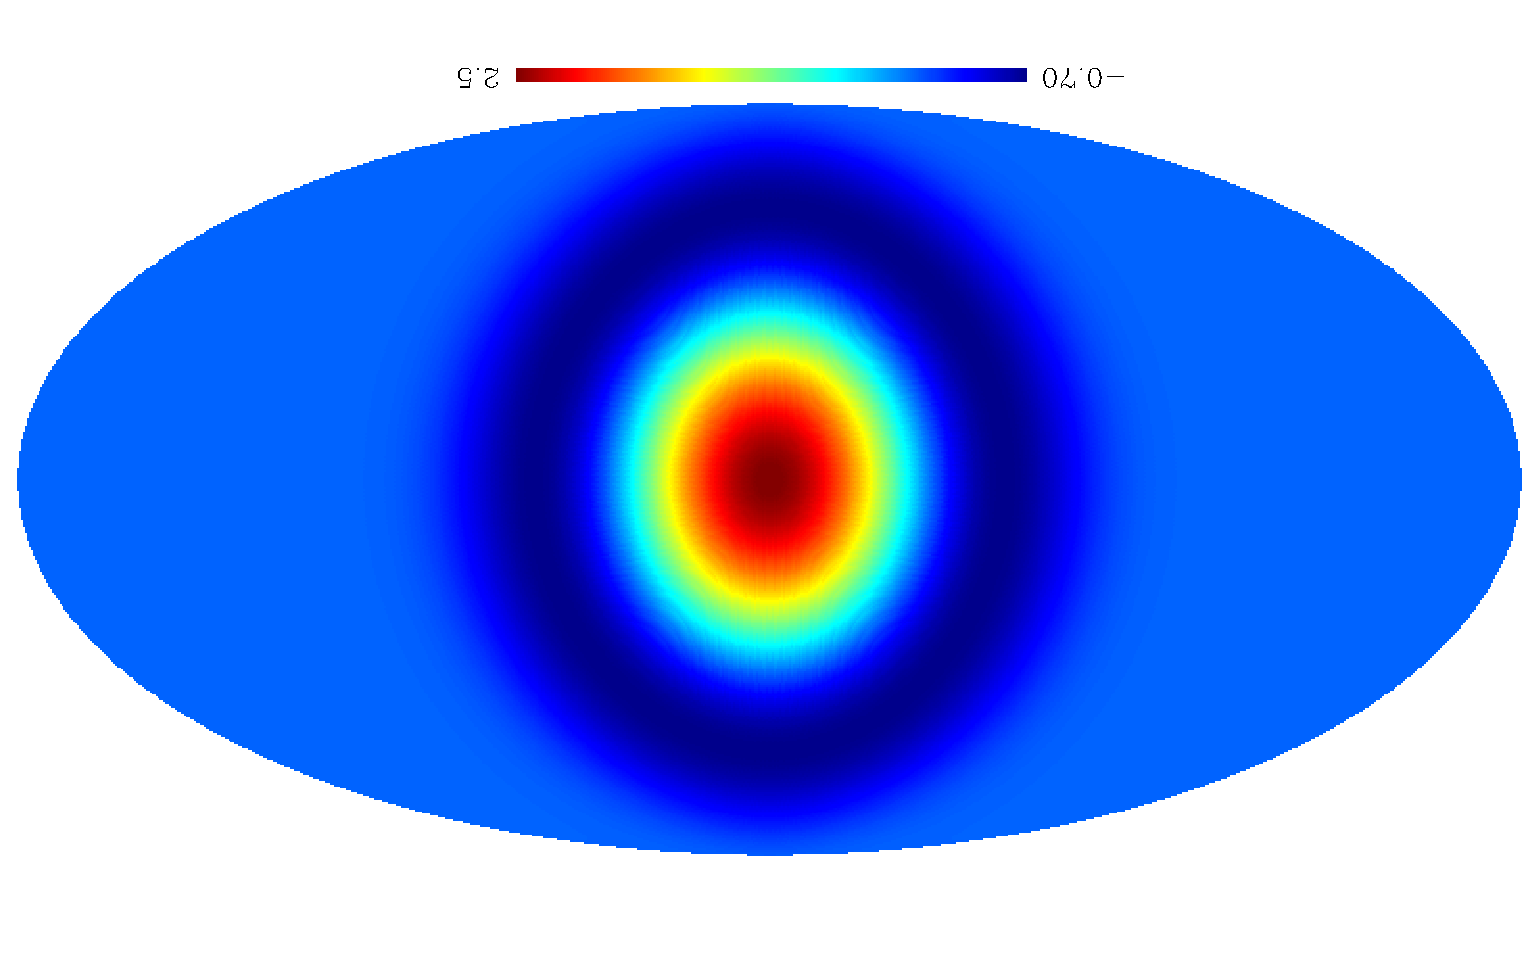
\includegraphics[angle=180,width=6.5cm]{wav_mex_hat_1.pdf}
}}\centerline{
\hbox{
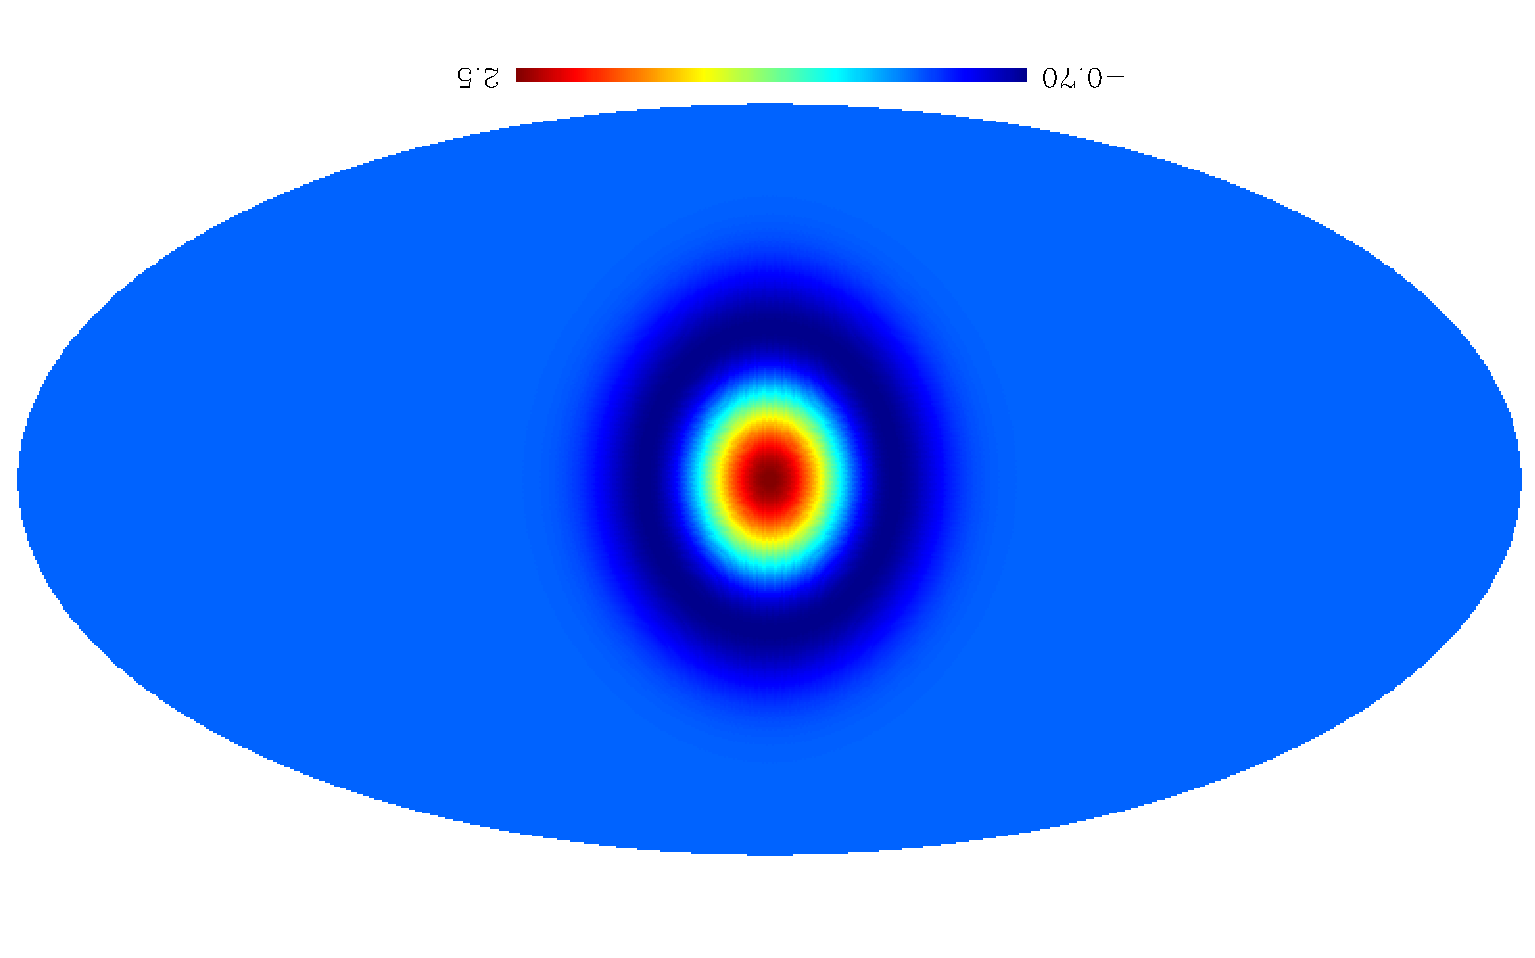
\includegraphics[angle=180,width=6.5cm]{wav_mex_hat_2.pdf}
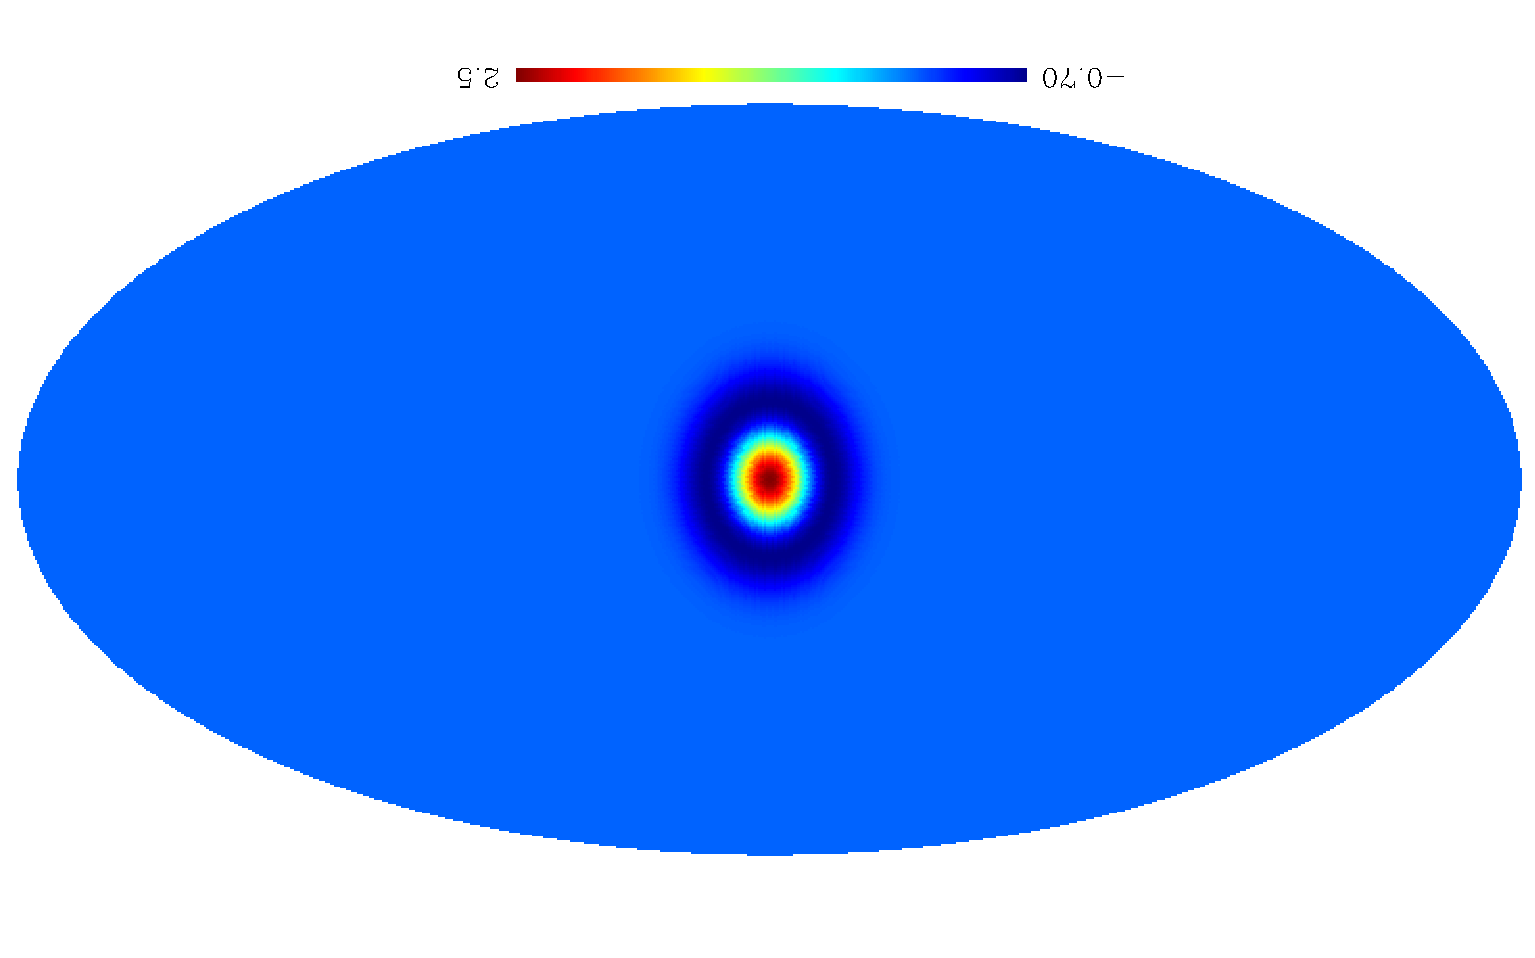
\includegraphics[angle=180,width=6.5cm]{wav_mex_hat_3.pdf}
}}
}
\caption{Mexican hat on the sphere for the dilation parameter equal to $a = \{1,2,4,8\}$.}
\label{fig_wav_mex_hat}
\end{figure}

% \begin{figure}[htb]
% \vbox{
% \centerline{
% \hbox{
% \includegraphics[angle=180,width=6.5cm]{mex_hat_0.pdf}
% \includegraphics[angle=180,width=6.5cm]{mex_hat_1.pdf}
% }}\centerline{
% \hbox{
% \includegraphics[angle=180,width=6.5cm]{mex_hat_8.pdf}
% \includegraphics[angle=180,width=6.5cm]{mex_hat_20.pdf}
% }}
% }
% \caption{Cosmic Microwave Background (CMB) simulated map and its mexican hat wavelet transform
% with dilation parameter $a = \{1,8,20\}$.}
% \label{fig_trans_cmb_wav_mex_hat}
% \end{figure}

The 2D Mexican hat wavelet transform is the second derivative of a Gaussian:
\begin{equation}
\label{rad_mexhat}
\psi(r) = \frac{1}{\sqrt{2 \pi}} \frac{1}{a} \Big( 2 - \Big( \frac{r}{a} \Big)^2 \Big) e^{- \frac{r^2}{2a^2}}
\end{equation}
where  $a$ is a scale factor parameter and $r$ the distance to the wavelet center.

Using the inverse stereographic projection, it is possible to extend the Mexican hat wavelet
on the sphere  \citep{wave:antoine99,wave:tenerio99,wave:cayon01,wave:holschneider96,wave:vielva04}:
\begin{equation}
\psi_a (r) = \frac{1}{\sqrt{2 \pi} C_a} \Big( 1 +  \Big( \frac{r}{2} \Big)^2 \Big)^2   \Big( 2 - \Big( \frac{r}{a} \Big)^2 \Big) e^{- \frac{r^2}{2a^2}},
\end{equation}
where $a$ is a scale factor, $C_a$ is a normalization term $C_a = a \Big( 1 + \frac{a^2}{2} + \frac{a^4}{4} \Big)^{\frac{1}{2}}$, and $r$ is the distance on the tangent plane, which is related to the polar angle $\theta$ through $r = 2 \textrm{tan} \frac{\theta}{2}$. This transform may be useful to analyze the data, but  it does not have a reconstruction operator, and can therefore not be used for restoration
applications.

Fig.~\ref{fig_wav_mex_hat} shows the Mexican hat wavelet on the sphere for  four different scales.
%  and Fig ~\ref{fig_trans_cmb_wa_mex_hat}  shows four scales for the a simulated CMB map.


\subsection{Directional Wavelets}
\label{dirwavelet}
\index{wavelet!directional wavelets}

% \index{sphere!directionnal wavelet}

\begin{figure}[htb]
\centering
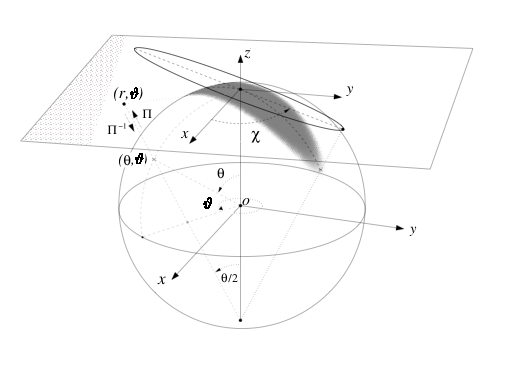
\includegraphics[width=9cm]{projection_stereo_ondelette_directionnelle.pdf}
\caption{Inverse stereographic projections  of a  directional wavelet on the sphere.}
\label{figprojstereo_direct2}
\end{figure}

To study anisotropic structures, the previously described continuous wavelet transform can be extended to directional wavelets  \citep{wave:antoine01,vielva06,McEwen08}.
Fig.~\ref{figprojstereo_direct2} shows the projection of an elliptic function from the plane to the sphere.  

\subsubsection{Elongated Mexican Hat Wavelet}
\index{Mexican hat!elongated}
\index{wavelet!Mexican hat}

\begin{figure}[htb]
\vbox{
\centerline{
\hbox{
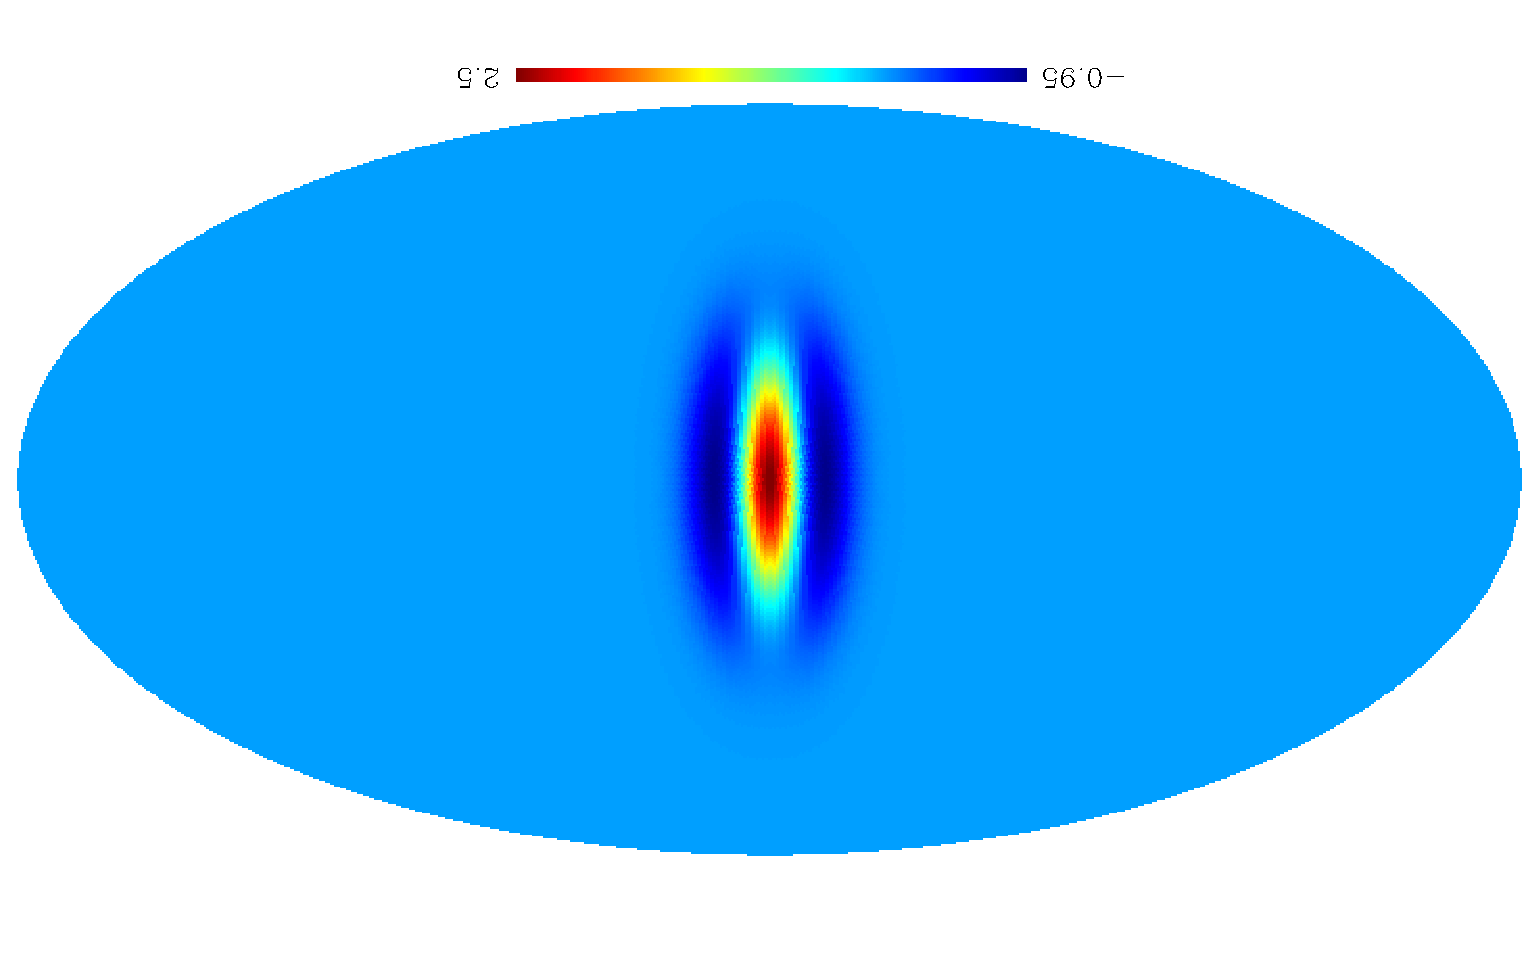
\includegraphics[angle=180,width=6.5cm]{dir_mex_hat_0.pdf}
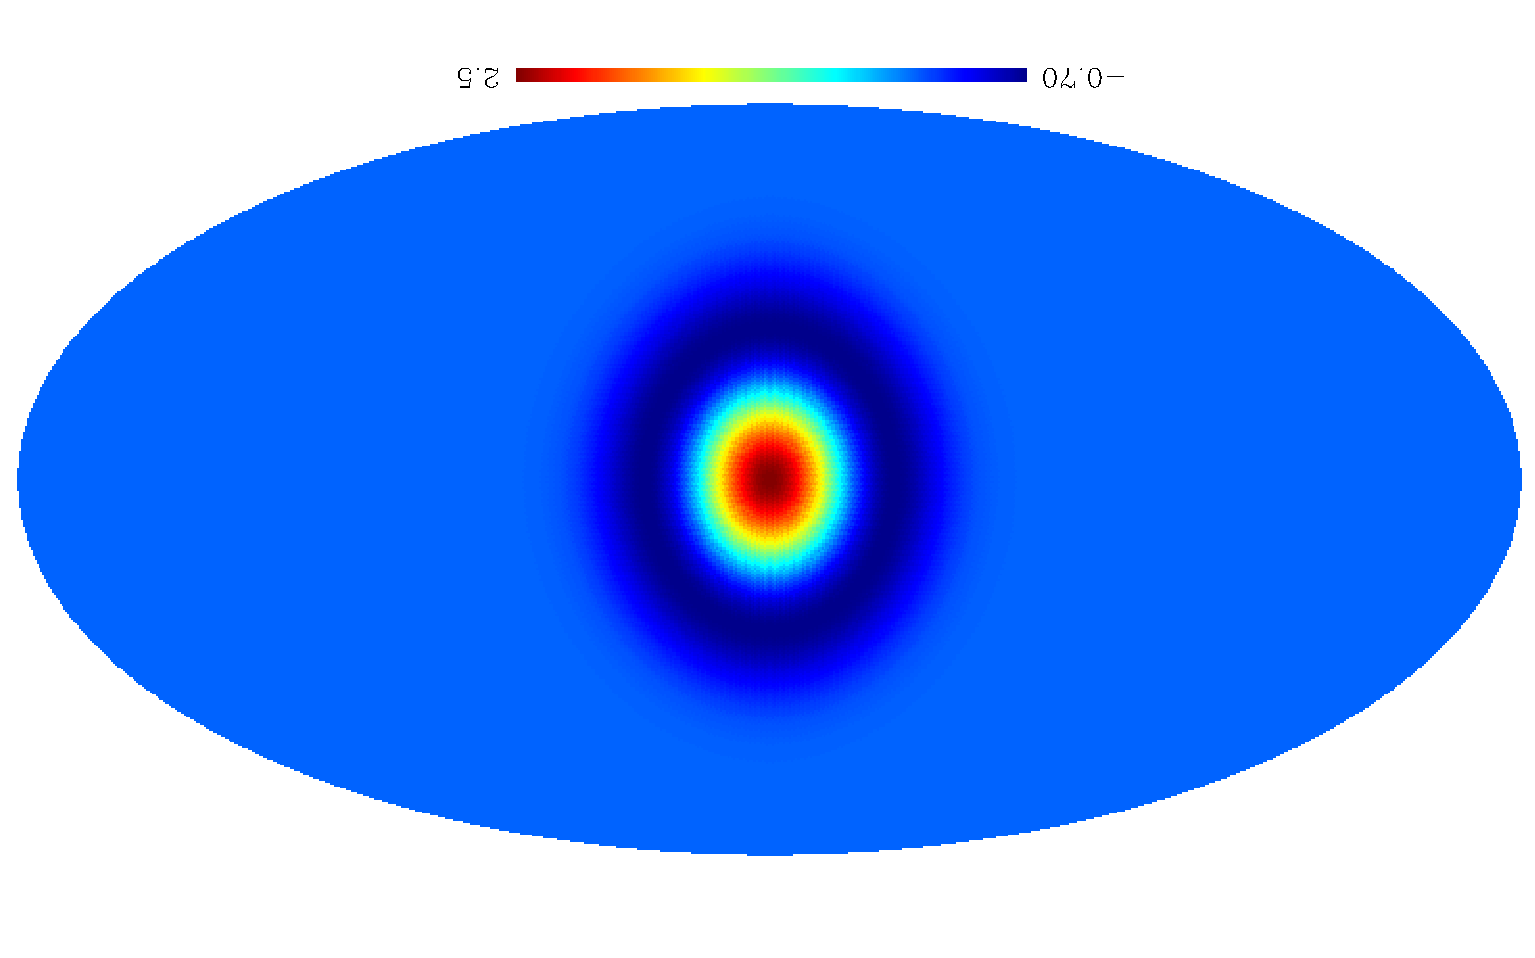
\includegraphics[angle=180,width=6.5cm]{dir_mex_hat_1.pdf}
}}\centerline{
\hbox{
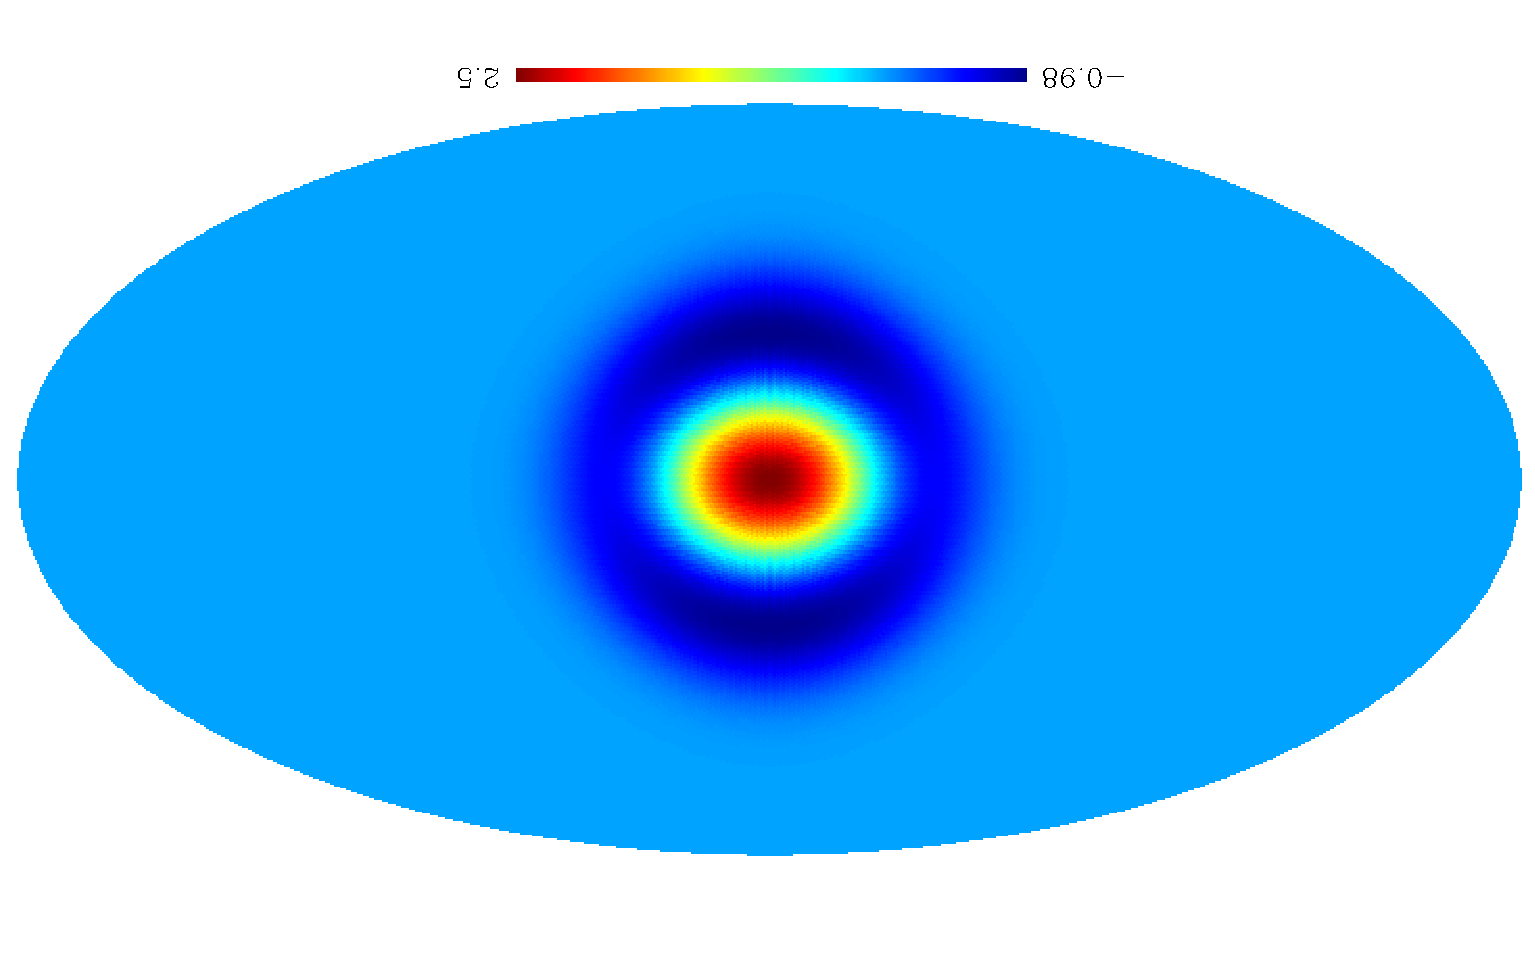
\includegraphics[angle=180,width=6.5cm]{dir_mex_hat_2.pdf}
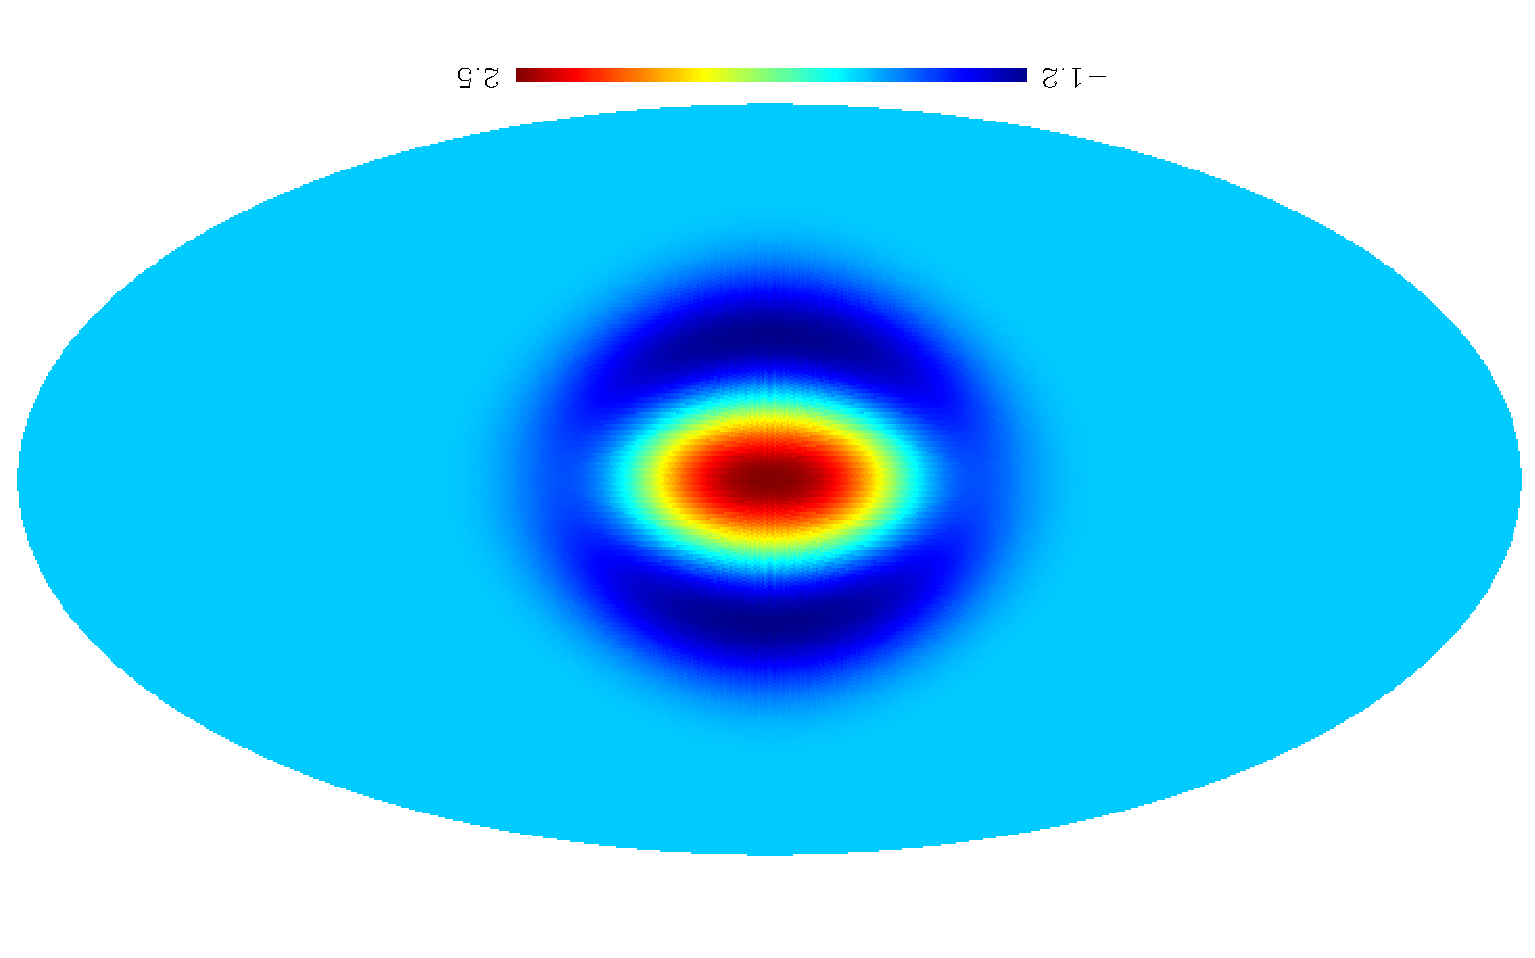
\includegraphics[angle=180,width=6.5cm]{dir_mex_hat_3.pdf}
}}
\centerline{
\hbox{
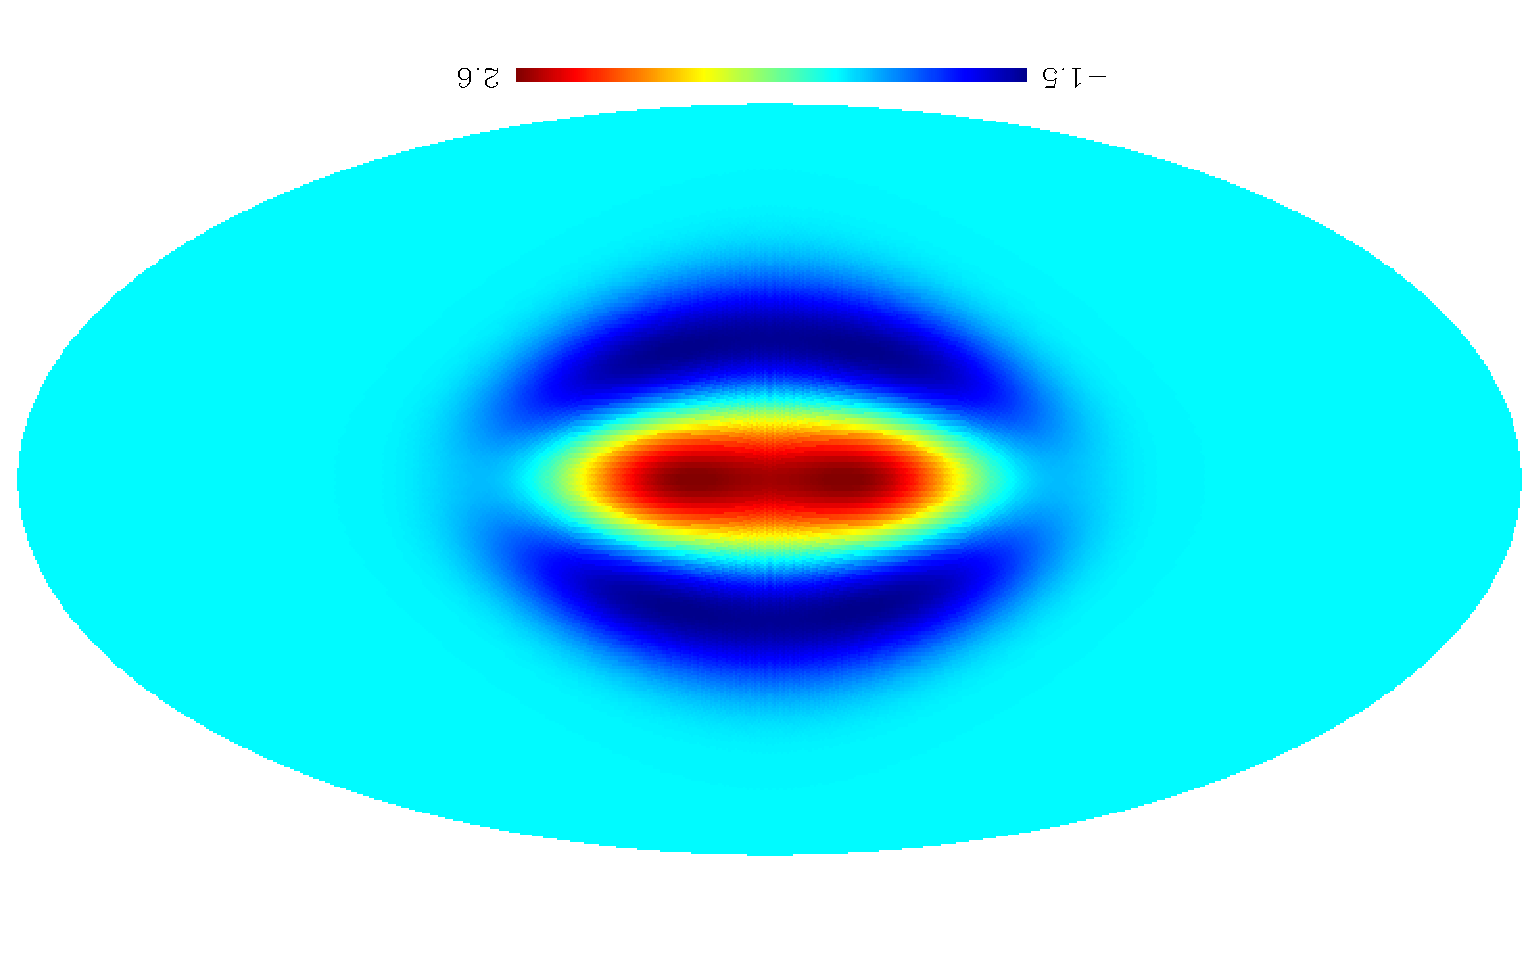
\includegraphics[angle=180,width=6.5cm]{dir_mex_hat_4.pdf}
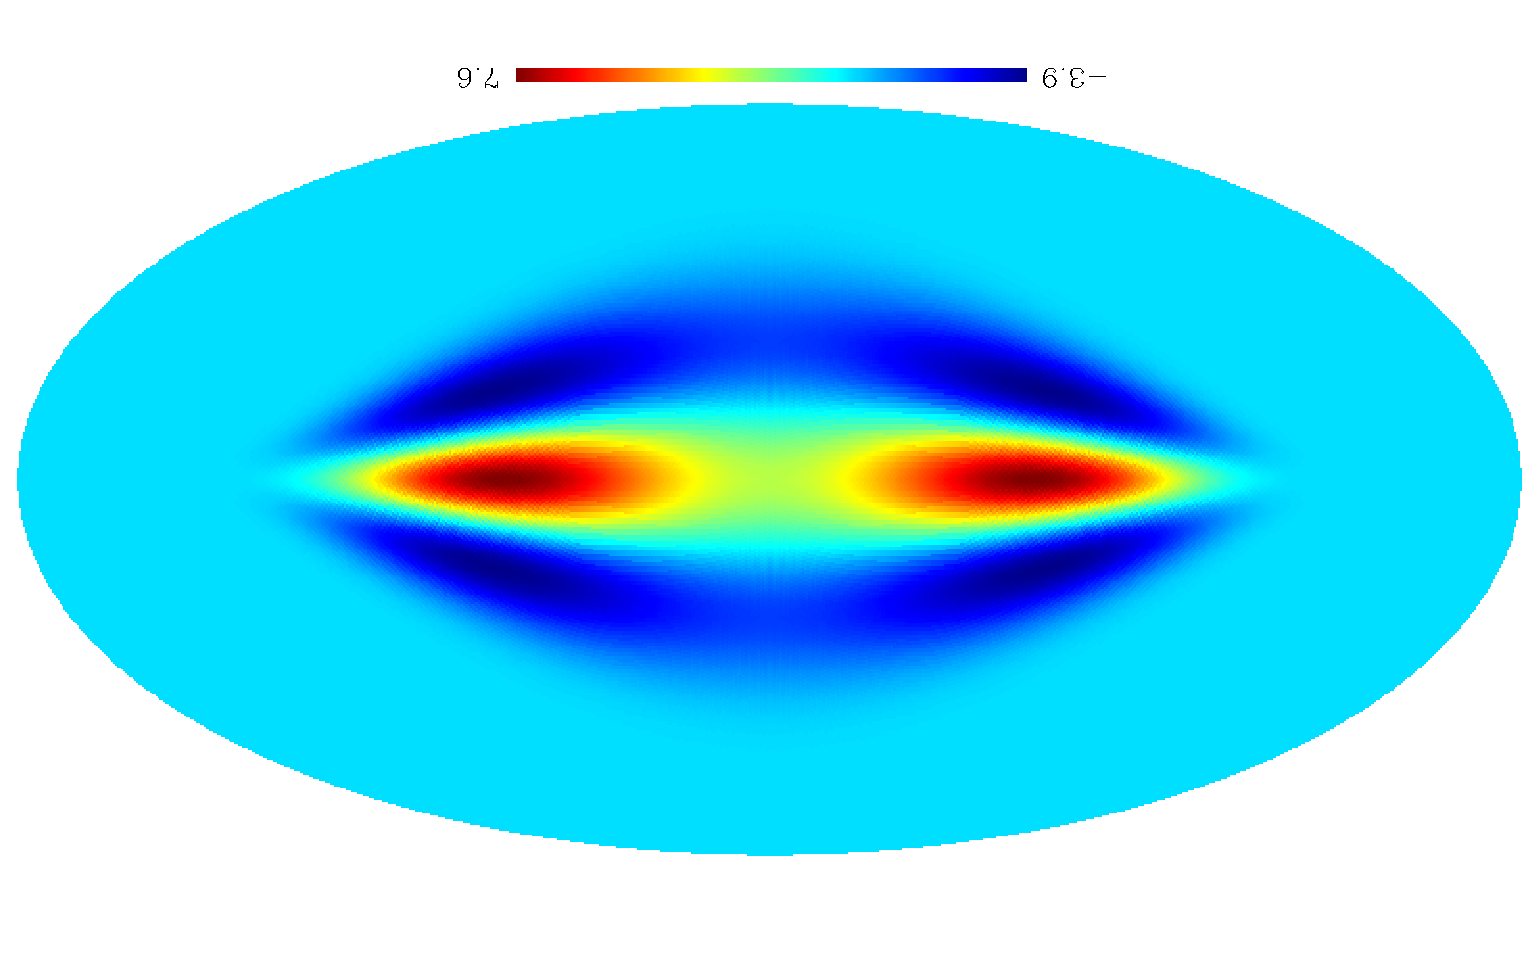
\includegraphics[angle=180,width=6.5cm]{dir_mex_hat_5.pdf}
}}
}
\caption{Elongated Mexican hat on the sphere for the dilation parameter equal to $a_x= 1$ and $a_y = \{0.5,1.,1.25,1.5,2,4\}$.}
\label{fig_dir_mex_hat}
\end{figure}

The elongated Mexican hat wavelet can be written as:
\begin{multline}
\label{directional_hat}
\psi_{a_x, a_y}(\theta, \vartheta) = \sqrt{\frac{2}{\pi}} C(a_x,a_y) \parenth{1+ \tan^2 \frac{\theta}{2}} \bigg( 1- \frac{4 \tan^2 \theta/2 }{a_x^2+a_y^2} \Big(\frac{a_y^2}{a_x^2} \cos^2 \vartheta \\
+  \frac{a_x^2}{a_y^2} \sin^2 \vartheta\Big) \bigg)  e^{-2 \tan \frac{\theta}{2}(\cos^2 \vartheta / a^2_x + \sin^2 \vartheta / a^2_y  )} ~,
\end{multline}
where $a_x$ and $a_y$ are the dilation factors along the two axes $O_x$ and $O_y$, $C(a_x,a_y)$ is a normalization constant defined as
\begin{eqnarray}
\label{directional_hat_norm}
C(a_x,a_y)& =& (a_x^2+a_y^2) \parenth{a_x a_y (3a_x^4+ 3a_y^4+2a_xa_y)}^{-1/2} ~.
\end{eqnarray}

Fig.~\ref{fig_dir_mex_hat} shows the wavelet functions for different dilation parameters $a_x$  and  $a_y$.


\subsubsection{Morlet Wavelet}
\index{wavelet!Morlet}

\begin{figure}[htb]
\vbox{
\centerline{
\hbox{
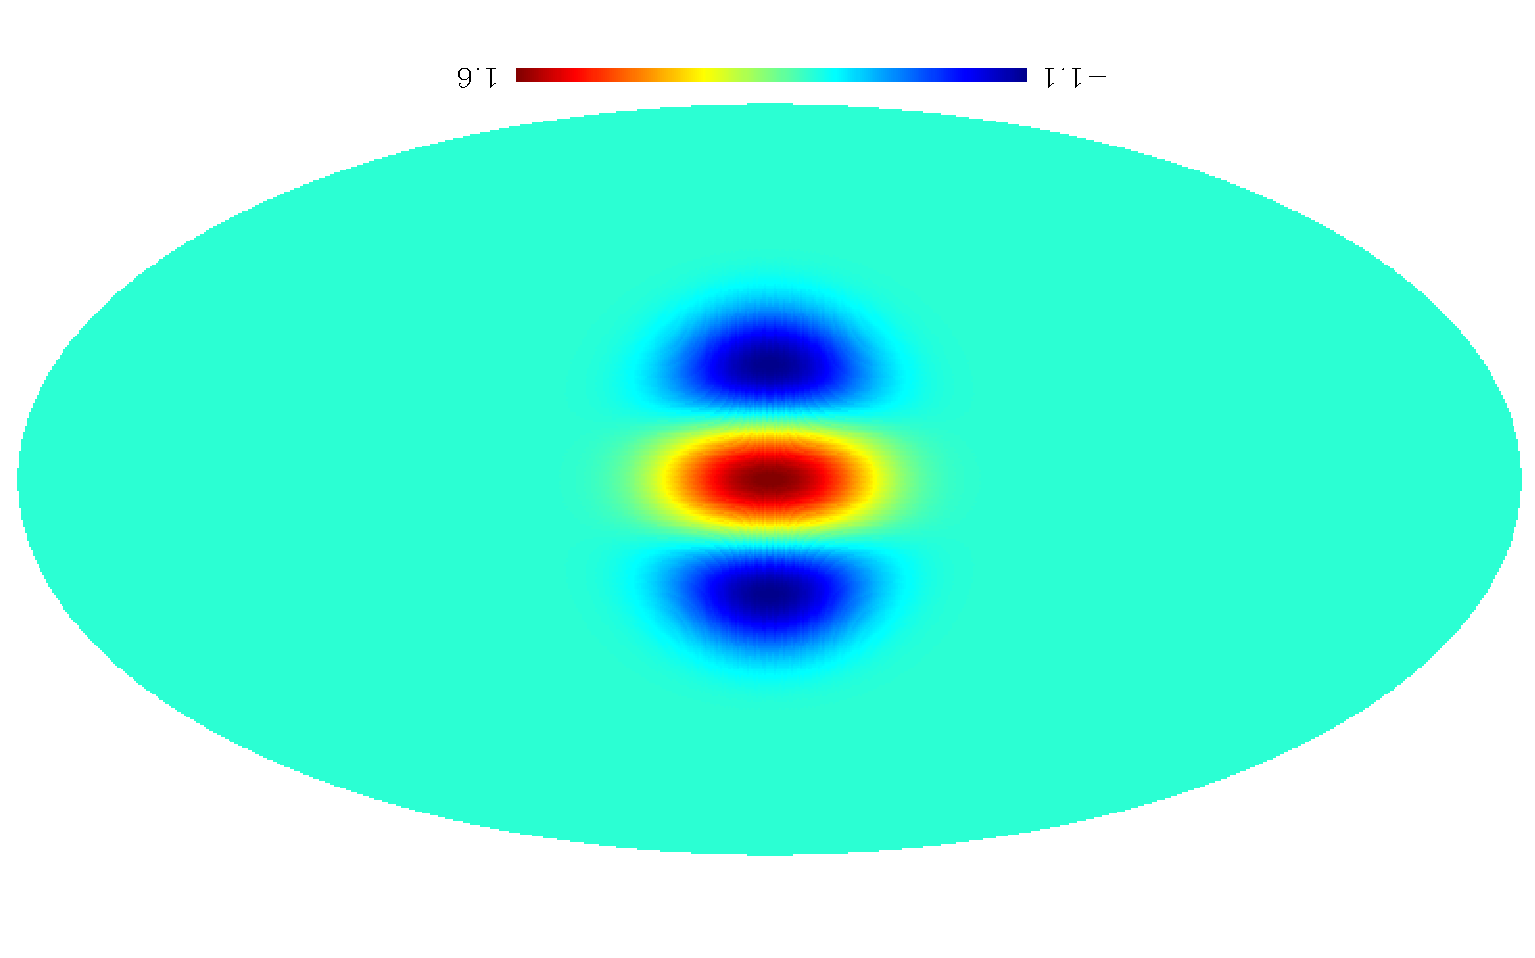
\includegraphics[angle=180,width=6.5cm]{dir_morlet_0.pdf}
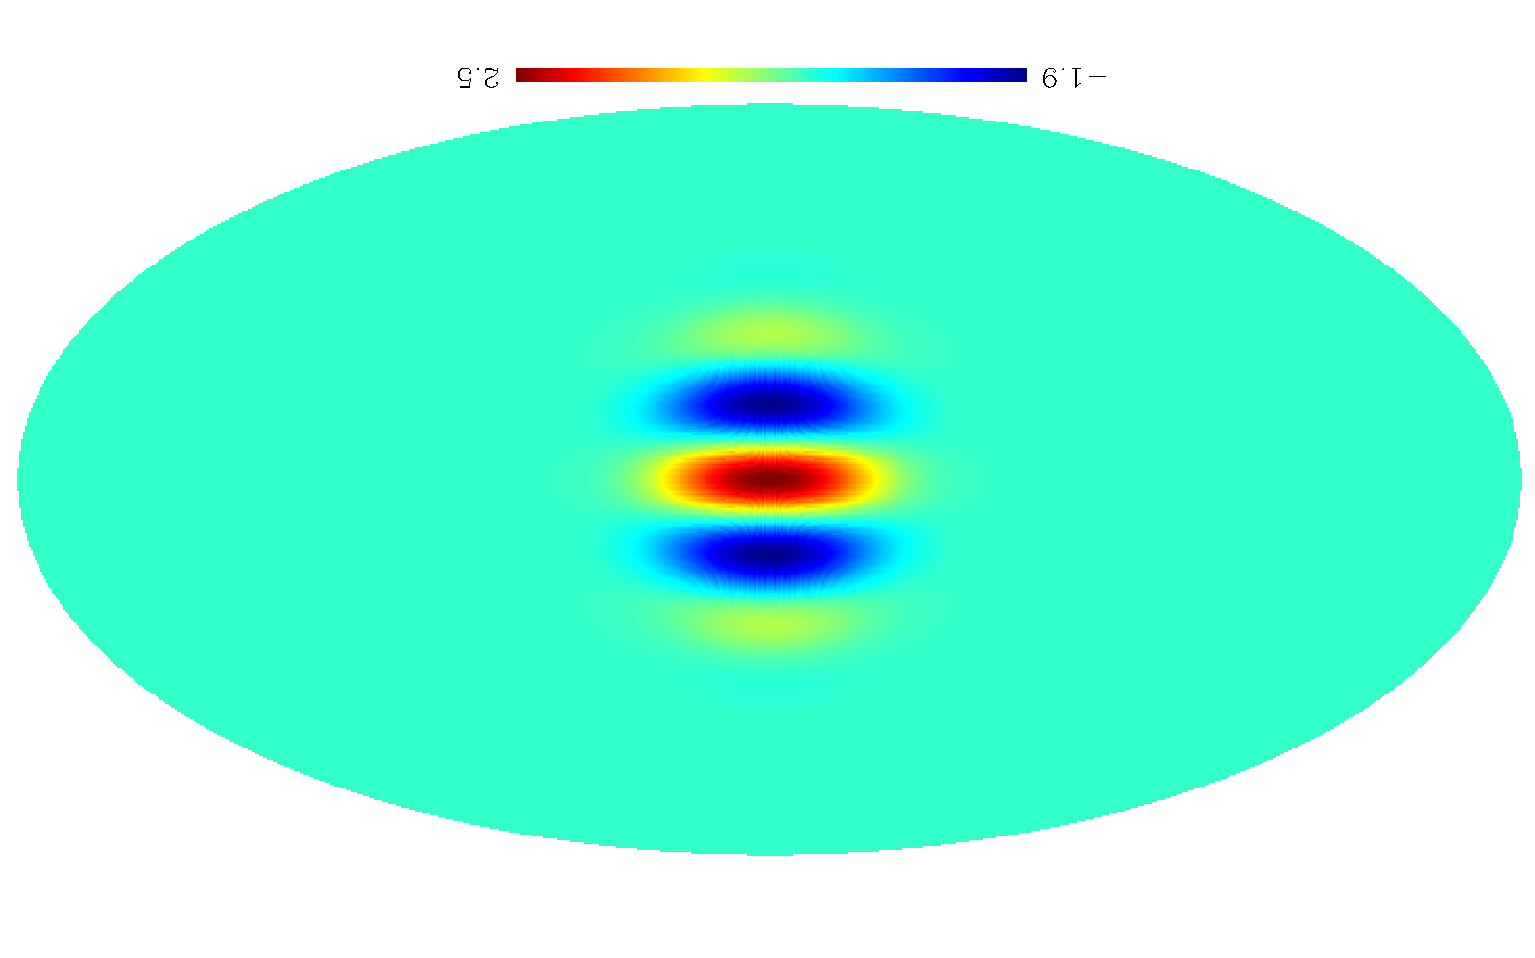
\includegraphics[angle=180,width=6.5cm]{dir_morlet_1.pdf}
}}\centerline{
\hbox{
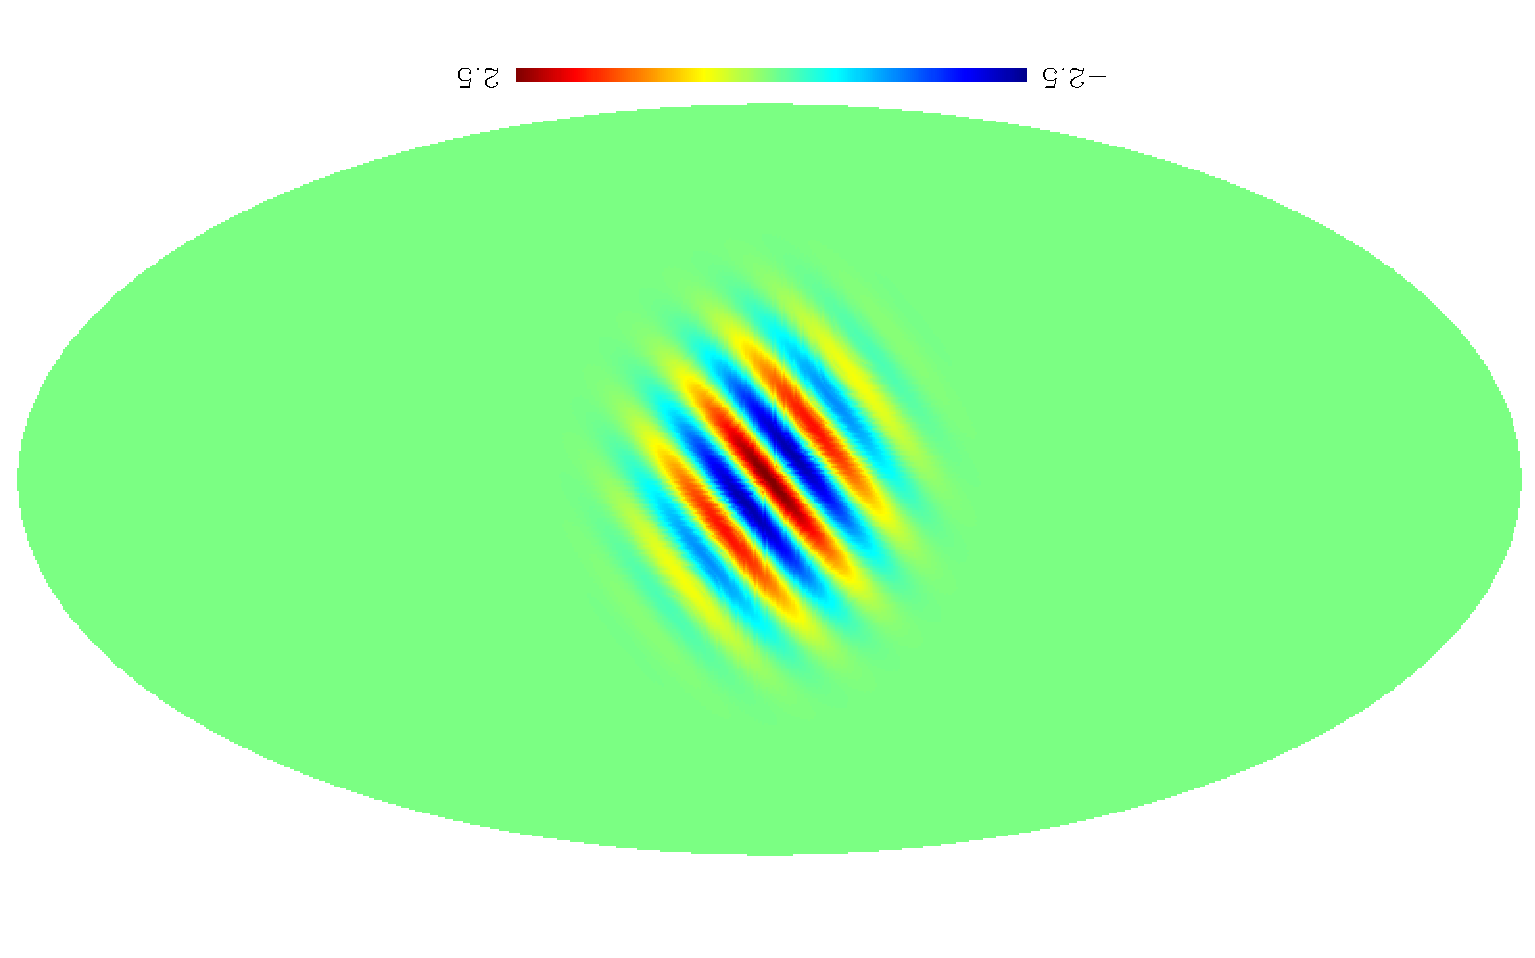
\includegraphics[angle=180,width=6.5cm]{dir_morlet_2.pdf}
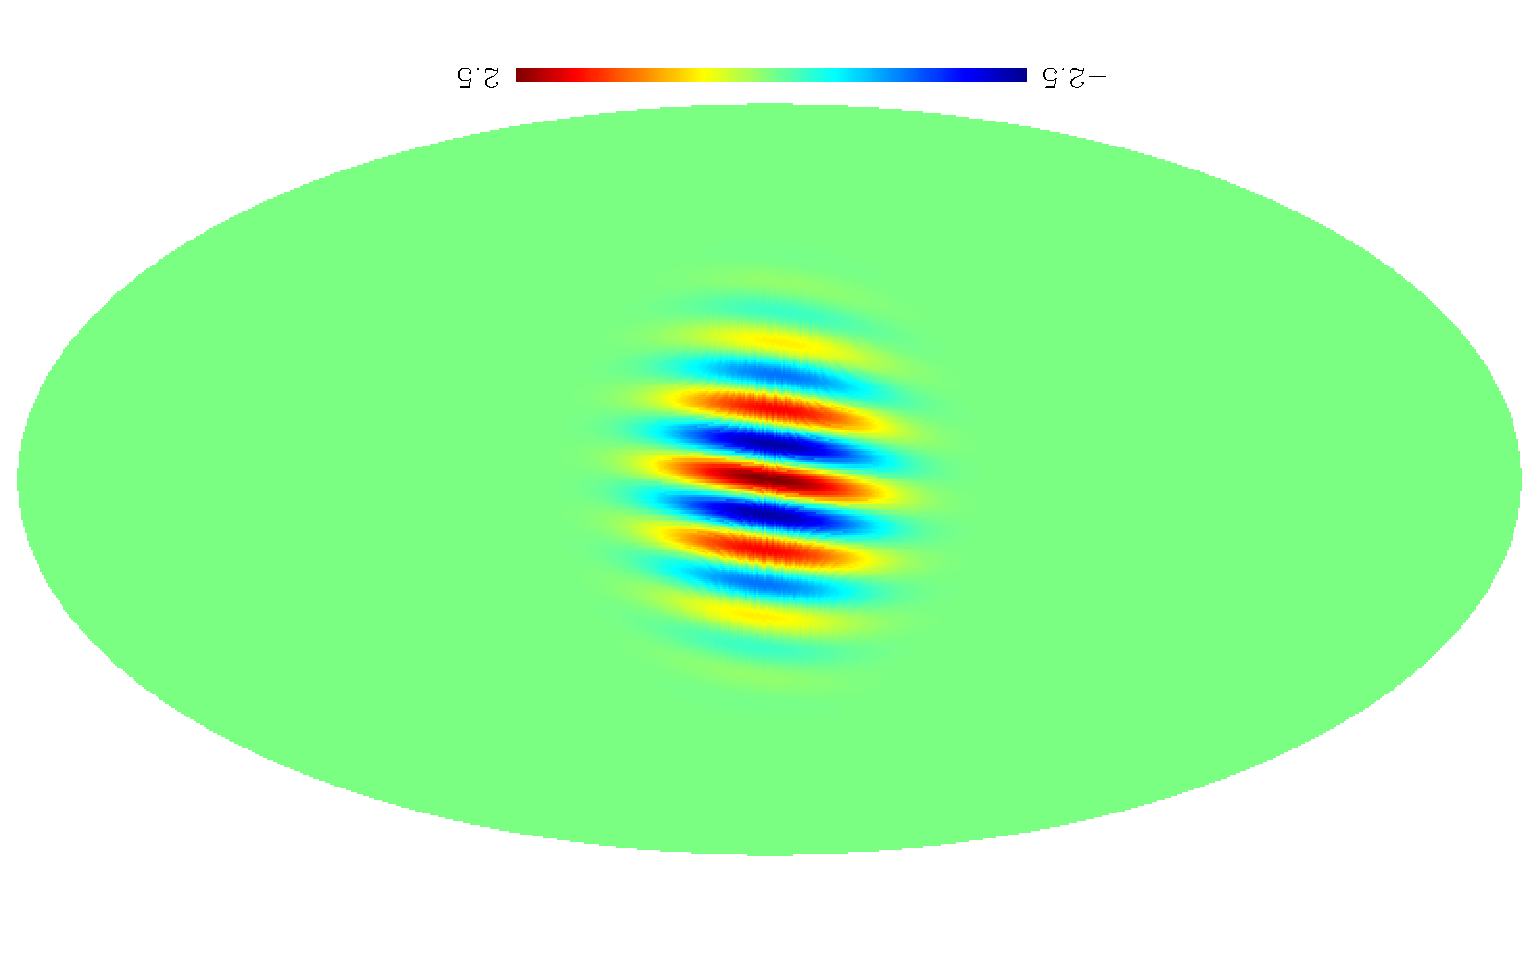
\includegraphics[angle=180,width=6.5cm]{dir_morlet_3.pdf}
}}
}
\caption{Morlet wavelets on the sphere for the parameter  $\bk$ equal to  (2,0), (4,0), (6,6) et (9,1).}
\label{fig_dir_morlet}
\end{figure}

The Morlet wavelet on the sphere, derived from the stereographic projection of the 2D function on the plane, is:
\begin{multline}
\label{real_morlet}
\psi_{a_x, a_y,  {\bf k}}(\theta, \vartheta)  =  \sqrt{\frac{2}{\pi}} C({\bf k}) (1+ \tan^2 \frac{\theta}{2}) \bigg(\cos \frac{  {\bf k} \cdotp  R^{-1} {\bf x} }{\sqrt{2}} \\  - e^{- |{\bf k}|^2/4} \bigg)  e^{-2 \tan^2(\theta/2)} 
\end{multline}
with $R^{-1}  {\bf x}  = (2 \tan (\theta/2) \cos \vartheta,2 \tan (\theta/2) \sin \vartheta)$,  ${\bf k}=(k_x,k_y)$, $|{\bf k}|^2 = k_x^2 + k_y^2$, 
 and  $C({\bf k}) = (1+3e^{-|{\bf k}|^2/2} -4e^{-3   |{\bf k}|^2/8})^{-1/2} $. ${\bf k}$ allows us to control the oscillations of the wavelet functions.
 
Fig.~\ref{fig_dir_morlet} shows the Morlet wavelet for ${\bf k}$  equal respectively to  $(2,0)$, $(4,0)$, $(6,6)$ and  $(9,1)$.

Continuous wavelet transforms have been intensively used in astrophysics, mainly to analyze the Cosmic Microwave Background  \citep{wave:vielva04}.
Directional wavelets based on steerable filters were also proposed in \citet{wiaux06,McEwen08}.
We present in the following a set of multiscale decompositions on the sphere which have a fast exact inverse transform, and are therefore suitable for many  applications such as restoration.
 
%===============================================================

\section{Redundant Wavelet Transform on the  Sphere with Exact Reconstruction}
\label{sect_wts}
%We show in this section that we can build  wavelet transforms on the sphere, based on the spherical harmonics transform, ewhich have an exact reconstruction and can therefore be easily used in different applications.


\subsection{Isotropic Undecimated Wavelet Transform on the Sphere}
Here an undecimated isotropic transform (UWTS) is described which is similar in many respects to the starlet transform (see Chapter~\ref{chp_uwt}), and will therefore be a good candidate for restoration applications.
Its isotropy is a favorable property when analyzing isotropic features. 
This isotropic transform is obtained using a scaling function ${\phi}_{l_c}(\theta, \vartheta)$ 
with cut-off frequency  $l_c$ and  azimuthal symmetry, meaning that ${\phi}_{l_c}$ does not depend 
on the azimuth $\vartheta$. Hence the spherical harmonics coefficients $\hat {\phi}_{l_c} [l,m]$ of ${\phi}_{l_c}$ vanish 
when $m \ne 0$ so that:
\begin{eqnarray}
{\phi}_{l_c}(\theta, \vartheta)= {\phi}_{l_c}(\theta) = \sum_{l = 0}^{l = l_c} \hat  {\phi}_{l_c} [l,0] Y_{l0}(\theta, \vartheta) .
\end{eqnarray}
Then, convolving a function $f(\theta, \vartheta) \in L_2(S^2)$ with ${\phi}_{l_c}$ is greatly simplified 
and the spherical harmonics coefficients of the resulting map $c_0$ are readily given by
\begin{eqnarray}
 \hat c_{0}[l,m] = \widehat{{\phi}_{l_c} * f} [l,m] = \sqrt{\frac{2l+1}{4\pi} } \hat {\phi}_{l_c} [l,0] \hat f[l,m]  .
\end{eqnarray}
\index{sphere!undecimated wavelet}

\subsubsection{From One Resolution to the Next}

A sequence of smoother approximations of $f$ on 
a dyadic resolution scale can be obtained using the scaling function ${\phi}_{l_c}$ as follows:
\begin{eqnarray}
\begin{split}
c_0   & = &  {\phi}_{ l_{c} }  \ast f        \\
c_1   & = &  {\phi}_{2^{-1} l_{c} }   \ast f    	   \\
&\ldots&\\ 
c_j    &=&   {\phi}_{2^{-j}  l_{c}  }  \ast f  ,
\end{split}
\end{eqnarray}
where ${\phi}_{2^{-j} l_{c} }$ is a rescaled version of ${\phi}_{l_{c}}$. The above multiresolution sequence can actually  be obtained recursively. 

Define a low pass filter $h_{j}$ for each scale $j$  by:
\begin{eqnarray}
 \widehat{H}_{j}[l,m]  & = & \sqrt{\frac{4\pi}{2l+1} }  \hat h_{j}[l,m]   \nonumber  \\
   &  = & 
   \begin{cases}
   \frac {   \hat \phi_{\frac{l_{c}}{2^{j+1}} }[l,m]   }   {  \hat  \phi_{  \frac{l_{c}}{2^{j}} }[l,m]   } & \mbox{if }  l  < \frac{ l_{c}} {2^{j+1}} \quad \textrm{and}\quad m = 0 , \\
   0 & \mbox{otherwise } . 
  \end{cases}
\end{eqnarray}
It is then easily shown that $c_{j+1}$ derives from $c_j$ by convolution on the sphere with $h_j$:  $c_{j+1} = c_{j} \ast h_j$.


\subsubsection{The Wavelet Coefficients}

Given an axisymmetric  wavelet function $\psi_{l_c}$, we can derive in the same way a 
high pass filter $g_j$ on each scale~$j$:
\begin{eqnarray}
 \widehat{G}_{j}[l,m]  & = & \sqrt{\frac{4\pi}{2l+1} }  \hat{g}_{j}[l,m] \nonumber  \\
   & = & 
  \begin{cases}
  \frac {   \hat \psi_{\frac{l_{c}}{2^{j+1}} }[l,m]   }   {  \hat  \phi_{  \frac{l_{c}}{2^{j}} }[l,m]   } & \mbox{if }  l  < \frac{ l_{c}} {2^{j+1}} \quad \textrm{and}\quad m = 0 ,\\
1 &\mbox{if }  l  \ge \frac{ l_{c}} {2^{j+1}} \quad \textrm{and}\quad m = 0 ,\\ 
0&  \mbox{otherwise } .
  \end{cases}
\end{eqnarray}
From this definition, the wavelet coefficients $w_{j+1} $ at scale $j+1$ are obtained from the previous scaling coefficients $c_j$ by a simple convolution on the sphere with $g_j$: $w_{j+1} = c_{j} \ast g_j$.

As in the  starlet transform   algorithm, the wavelet coefficients can be defined as the difference between two consecutive resolutions, $w_{j+1}(\theta, \vartheta) = c_{j}(\theta, \vartheta) - c_{j+1}(\theta, \vartheta)$. This defines a zonal wavelet function $\psi_{l_c}$ as:
\begin{eqnarray}\label{wavelet}
\hat \psi_{\frac{l_c}{2^{j}}}[l,m] = \hat \phi_{\frac{l_c}{2^{j-1}}} [l,m]  - \hat \phi_{\frac{l_c}{2^{j}}}[l,m] .
\end{eqnarray}
The high pass filters $g_j$ associated with this wavelet are expressed as: 
\begin{eqnarray}
\begin{split}
\widehat{G}_{j}[l,m]  & = \sqrt{\frac{4\pi}{2l+1} } \hat{g}_{j}[l,m]  \\
                  & = 1 - \sqrt{\frac{4\pi}{2l+1} } \hat{h}_j[l,m]   =   1 - \widehat{H}_j[l,m] .
\end{split}
\end{eqnarray}
Obviously other wavelet functions could be used just as well.


\subsubsection{Choice of the Scaling Function}
Any function with a cut-off frequency is a possible candidate. We retained here 
a B-spline function of order 3 (see Chapter~\ref{chp_uwt}):
\begin{eqnarray}
{\hat{\phi}}_{l_c} [l,m] = \frac{3}{2} B_{3}  \left(  \frac{2l}{l_{c}} \right)
\end{eqnarray}
where $B_3(t)$ is the scaling function defined in Section~\ref{sect_starlet}.
%\[B_3(t) = \frac{1}{12}({\mid{t-2}\mid}^3 - 4 {\mid{t-1}\mid}^3 + 6 {\mid{t}\mid}^3 - 4 {\mid{t+1}\mid}^3 + {\mid{t+2}\mid}^3)  \]


\begin{figure}[htb]
\vbox{
\centerline{
\hbox{
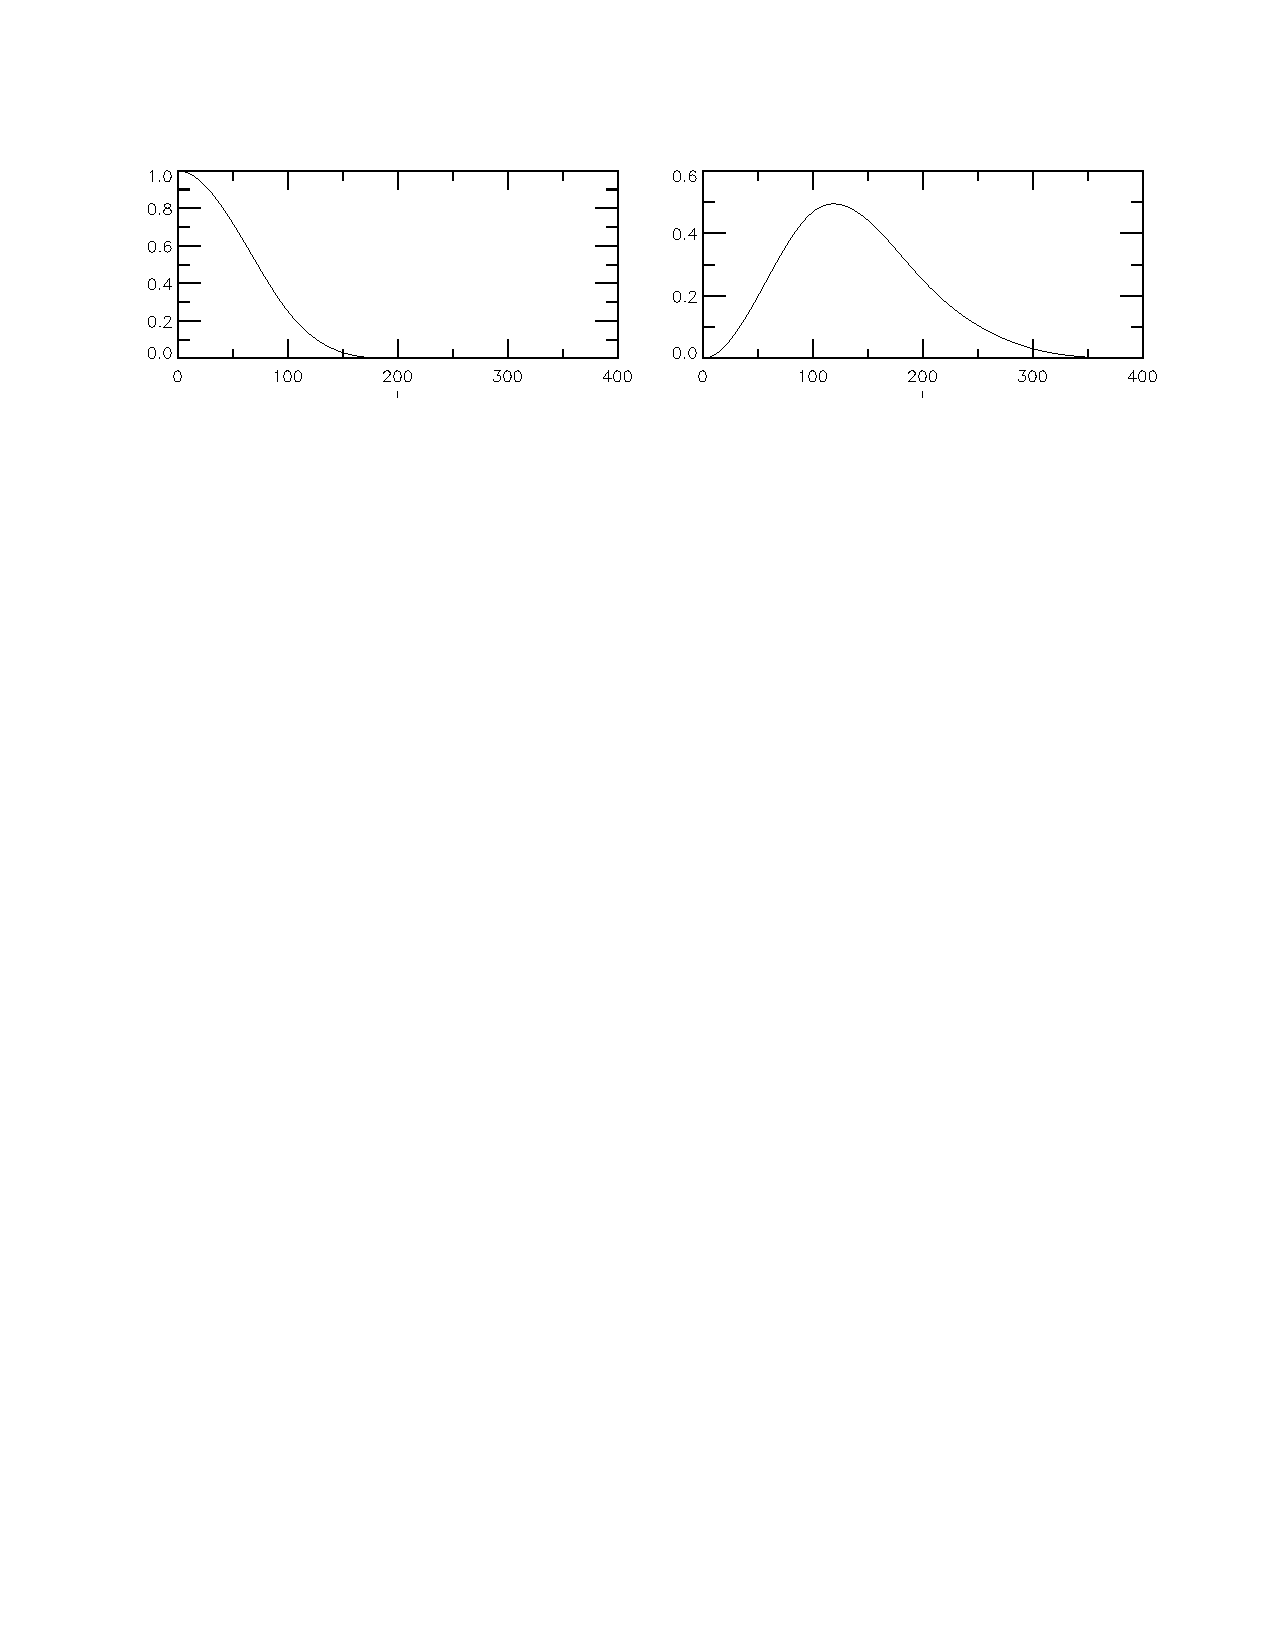
\includegraphics[width=14cm,height=4.5cm]{fig_sphere_filterbank1.pdf}
% 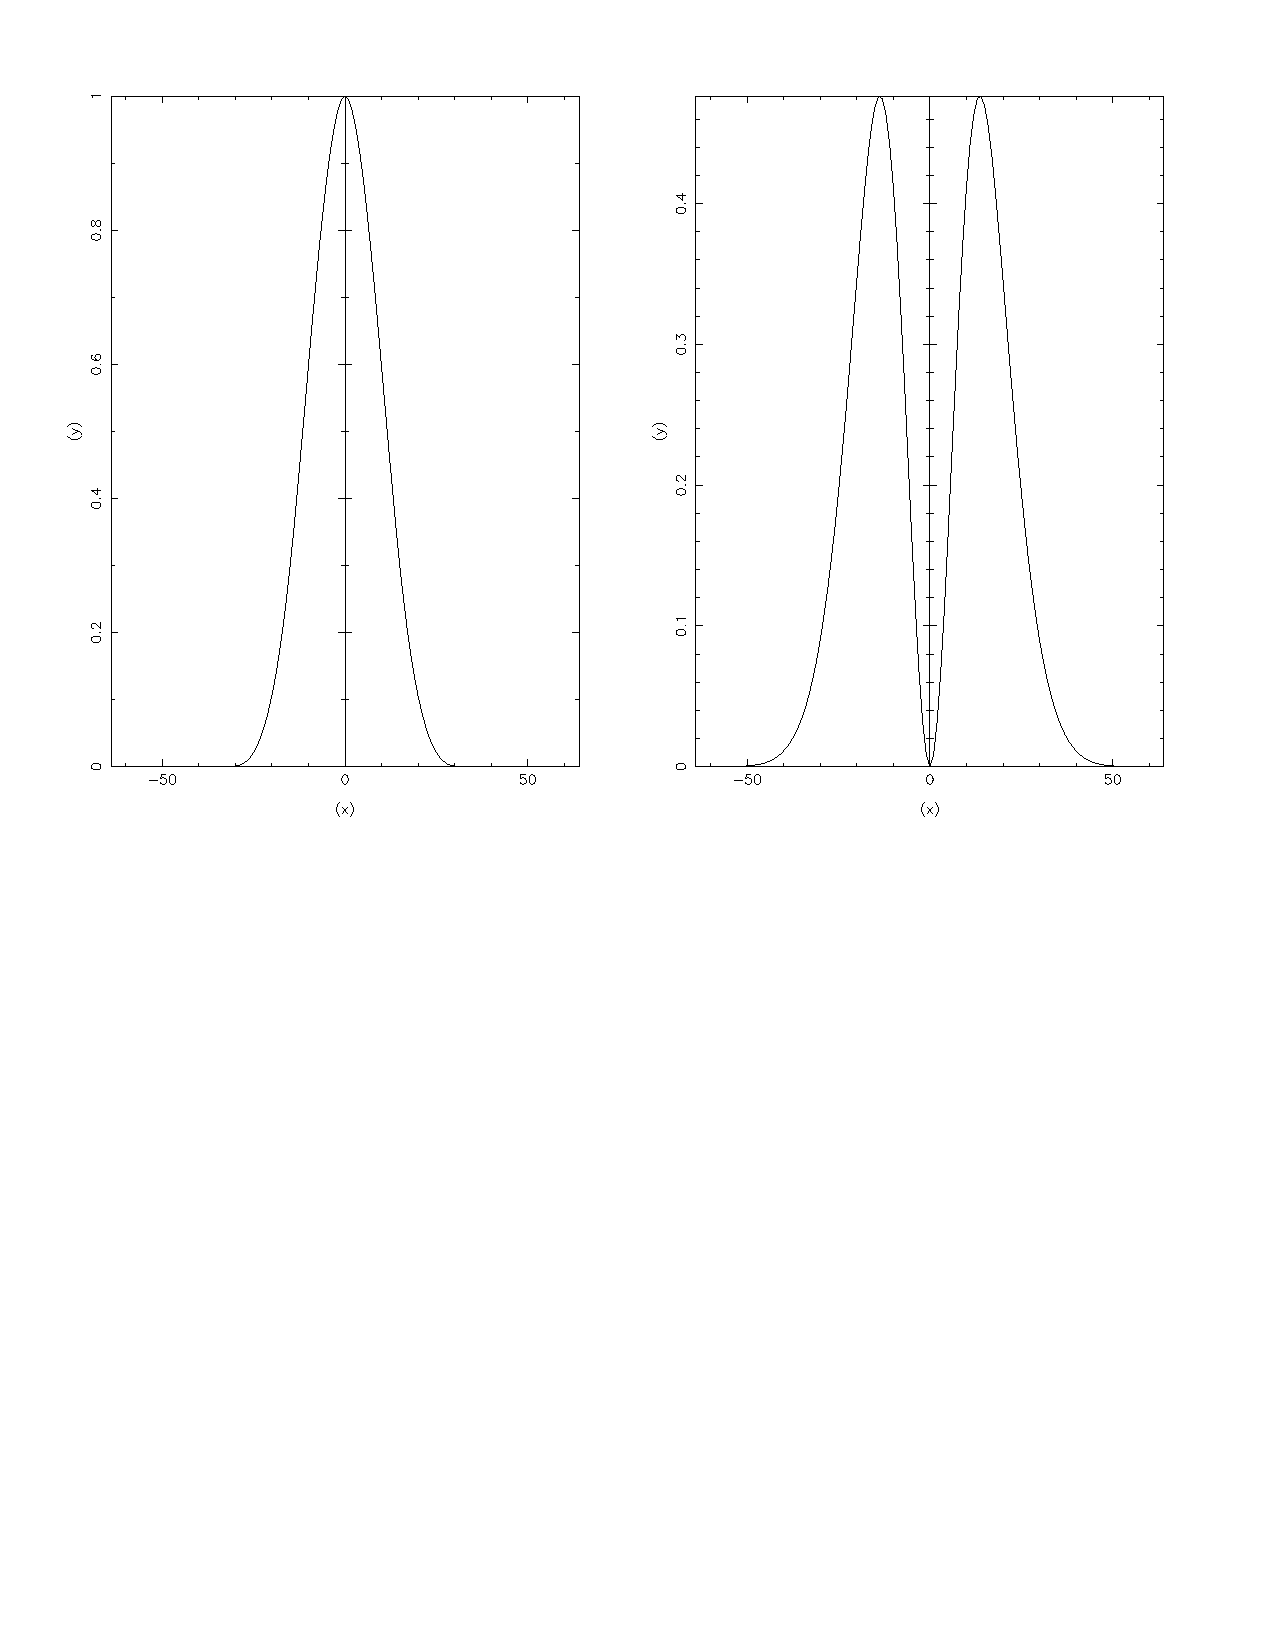
\includegraphics[width=14cm,height=5cm]{ch1_diff_uv_phi_psi.pdf}
}}}
\caption{On the left, spherical harmonics coefficients $\hat{{\phi}}[l,0]$ of the the scaling function ${{\phi}}$ and, on the right, those of the wavelet function ${\psi}$.}
\label{fig_diff_uv_phi_psi}
\end{figure}

In Fig.~\ref{fig_diff_uv_phi_psi} the spherical harmonics coefficients of the scaling function derived from a B$_3$-spline, and those of the associated wavelet function \eqref{wavelet}, are plotted as a function of $l$. Other functions such as the needlet function \citep{marinucci08} can be used as well.

The steps of the UWT on the sphere of a discrete image $X$ sampled from $f$ are summarized in Algorithm~\ref{algo_uwts}. If the wavelet function corresponds to the choice \eqref{wavelet}, Step 3 in this UWTS algorithm reduces to $w_{j+1} = c_{j} - c_{j+1}$.

% Their corresponding conjugate low pass and high pass filters $h$ and $g$ are plotted in Fig.~\ref{fig_diff_uv_ht_gt}. 

{\linespread{1}
\begin{algorithm}[h]
\caption{The Undecimated Wavelet Transform on the Sphere.}
\label{algo_uwts}
\noindent{\bf Task:} Compute the UWTS of a discrete $X$.\\
\noindent{\bf Parameters:} Data samples $X$ and number of of wavelet scales $J$.\\  
\noindent{\bf Initialization:} 
\begin{itemize}
\item $c_0=X$.
\item Compute the B$_3$-spline scaling function and derive $\hat{\psi}$, $\widehat{H}$ and $\widehat{G}$ numerically.
\item Compute the corresponding spherical harmonics transform of $c_0$.
\end{itemize}
\For{$j=0$ to $J-1$} {
\begin{enumerate}[1.]
\item Compute the spherical harmonics transform of the scaling coefficients:  $\hat{c}_{j+1}=\hat{c}_j\widehat{H}_{j}$.
\item Compute the inverse spherical harmonics transform of $\hat{c}_{j+1}$ to get $c_{j+1}$.
\item Compute the spherical harmonics transform of the wavelet coefficients:  $\hat{w}_{j+1}=\hat{c}_j\widehat{G}_{j}$.
\item Compute the inverse spherical harmonics transform of $\hat{w}_{j+1}$ to get $w_{j+1}$.
\end{enumerate}
}
\noindent{\bf Output:} ${\cal W}=\{w_1, w_2, \dots, w_{J}, c_{J}\}$ the UWTS of $X$.
\end{algorithm}
}

\begin{figure}[htb]
\vbox{
\centerline{
\hbox{
 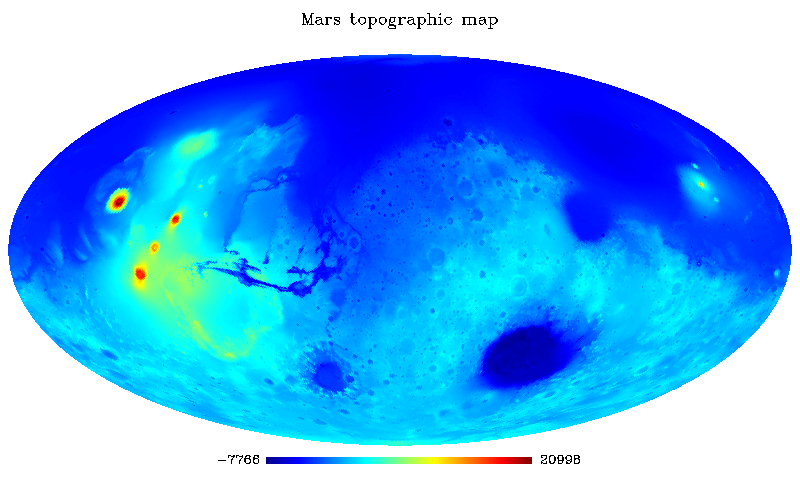
\includegraphics[width=6.5cm,height=3.9cm]{fig_mars.png}
 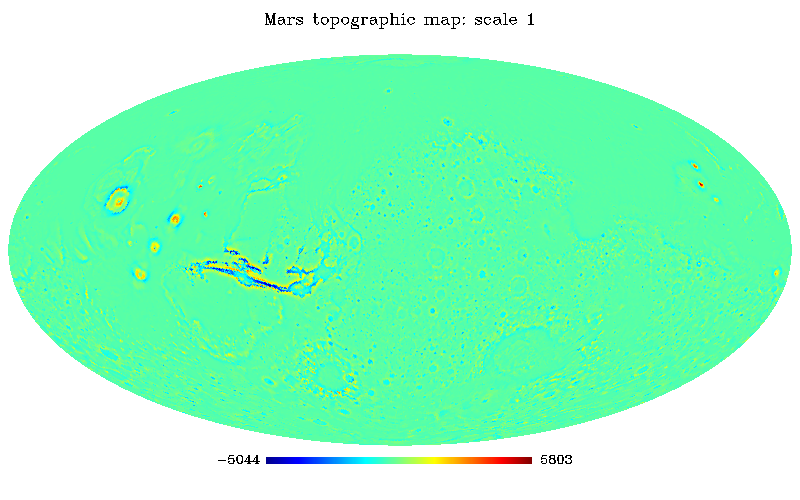
\includegraphics[width=6.5cm,height=3.9cm]{fig_mars_scale1.png}
}}
\centerline{
\hbox{
 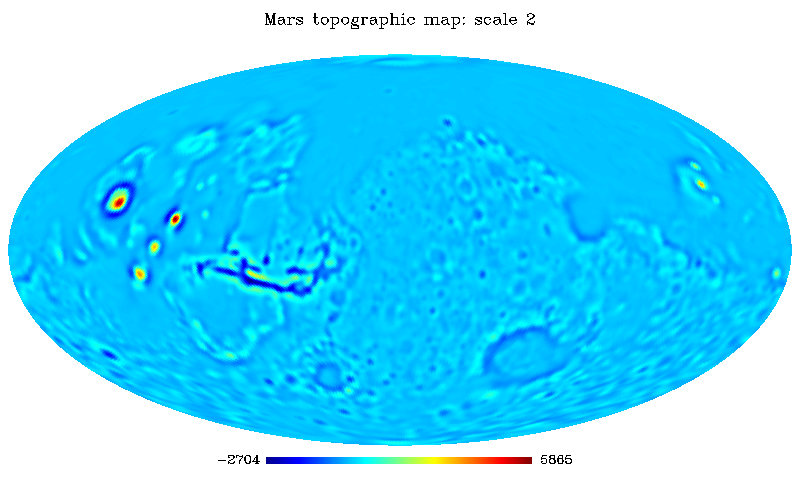
\includegraphics[width=6.5cm,height=3.9cm]{fig_mars_scale2.png}
 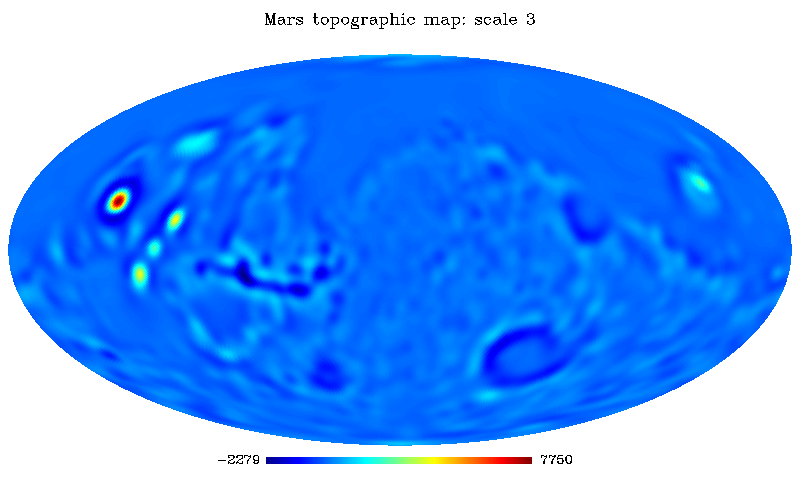
\includegraphics[width=6.5cm,height=3.9cm]{fig_mars_scale3.png}
}}
\centerline{
\hbox{
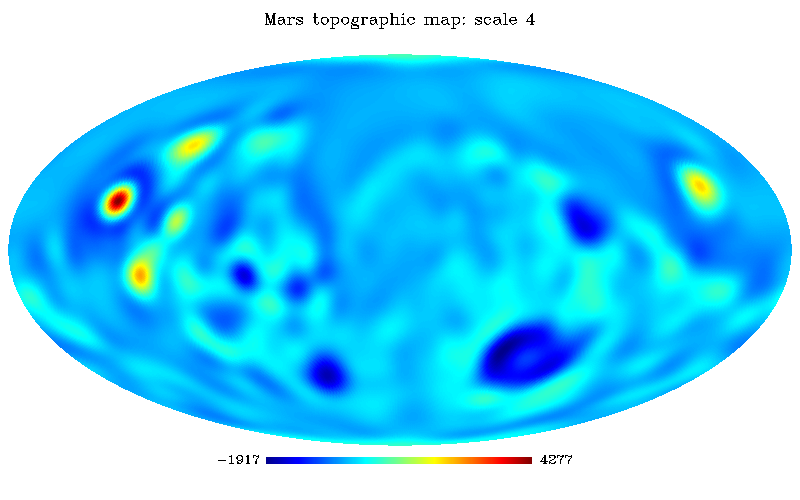
\includegraphics[width=6.5cm,height=3.9cm]{fig_mars_scale4.png}
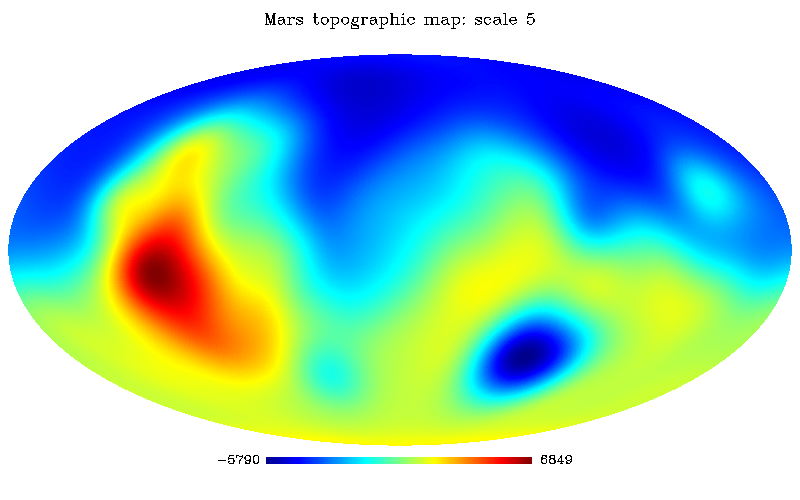
\includegraphics[width=6.5cm,height=3.9cm]{fig_mars_scale5.png}
}}
}
\caption{Mars topographic map and its UWTS (four wavelet detail scales and the scaling (smooth) band).}
\label{Figure:UWTS}
\index{data!Mars topography}
\end{figure}

Fig.~\ref{Figure:UWTS} shows the Mars topographic map (top left)
\footnote{The Mars Orbiter Laser Altimeter (MOLA) generated altimetry profiles used to create global topographic maps. The MOLA instrument stopped acquiring altimetry data on June 30, 2001, and after that operated in passive radiometry mode until the end of the Mars Global Surveyor mission. MOLA data sets are produced by the MOLA Science Team and archived by the PDS Geosciences Node.} and its wavelet transform, using five scales (four wavelet scales + coarse scale). The sum of the five scales reproduces exactly the original image.
\index{Mars Orbiter Laser Altimeter}

\subsubsection{Inverse Transform}

If the wavelet is the difference between two resolutions, a straightforward reconstruction of an image from its wavelet coefficients ${\cal W} = \{w_1,\dots, w_{J}, c_{J}\}$ is: 

\begin{eqnarray}
 c_{0}(\theta, \vartheta) = c_{J}(\theta, \vartheta) + \sum_{j=1}^J  w_j(\theta, \vartheta) .
\end{eqnarray}
This reconstruction formula is the same as with the starlet algorithm.

\begin{figure}[htb]
\vbox{
\centerline{
\hbox{
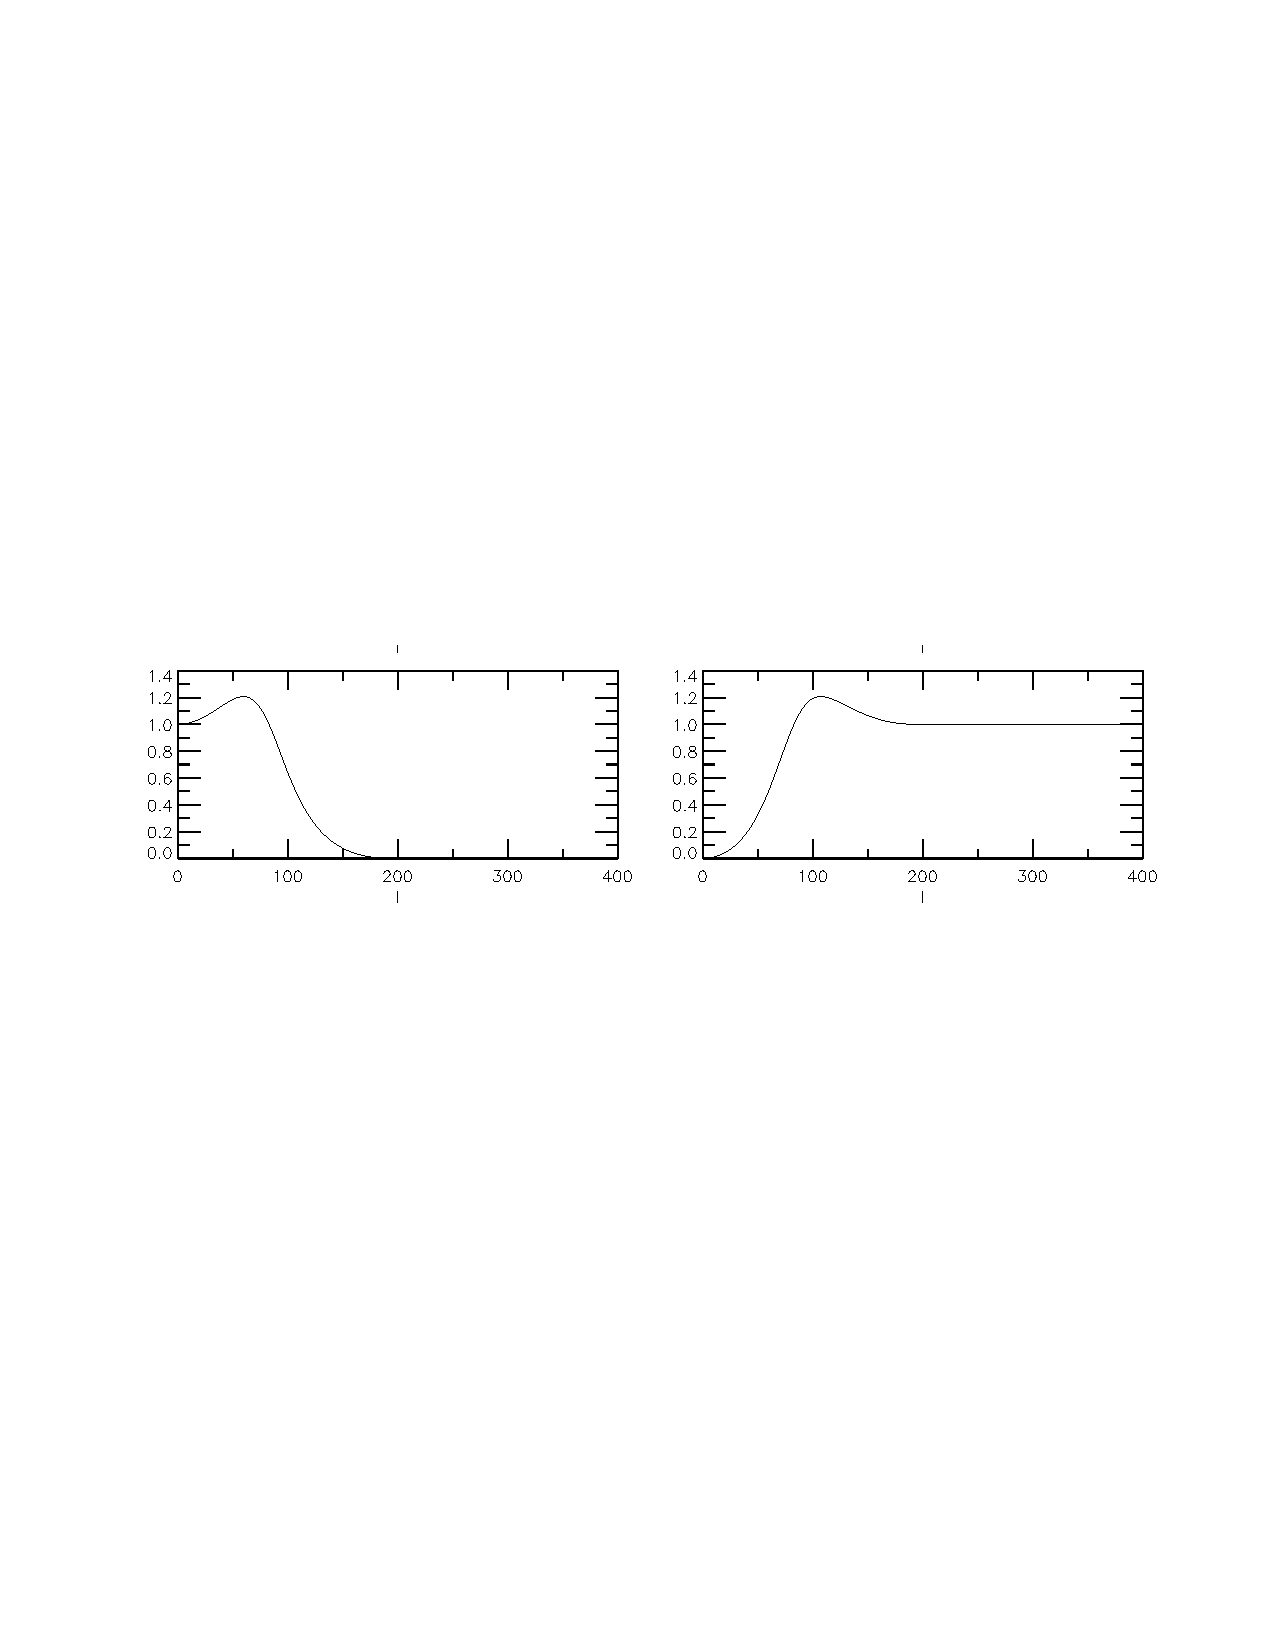
\includegraphics[width = 13cm, height = 4.cm]{fig_sphere_filterbank2.pdf} 
% 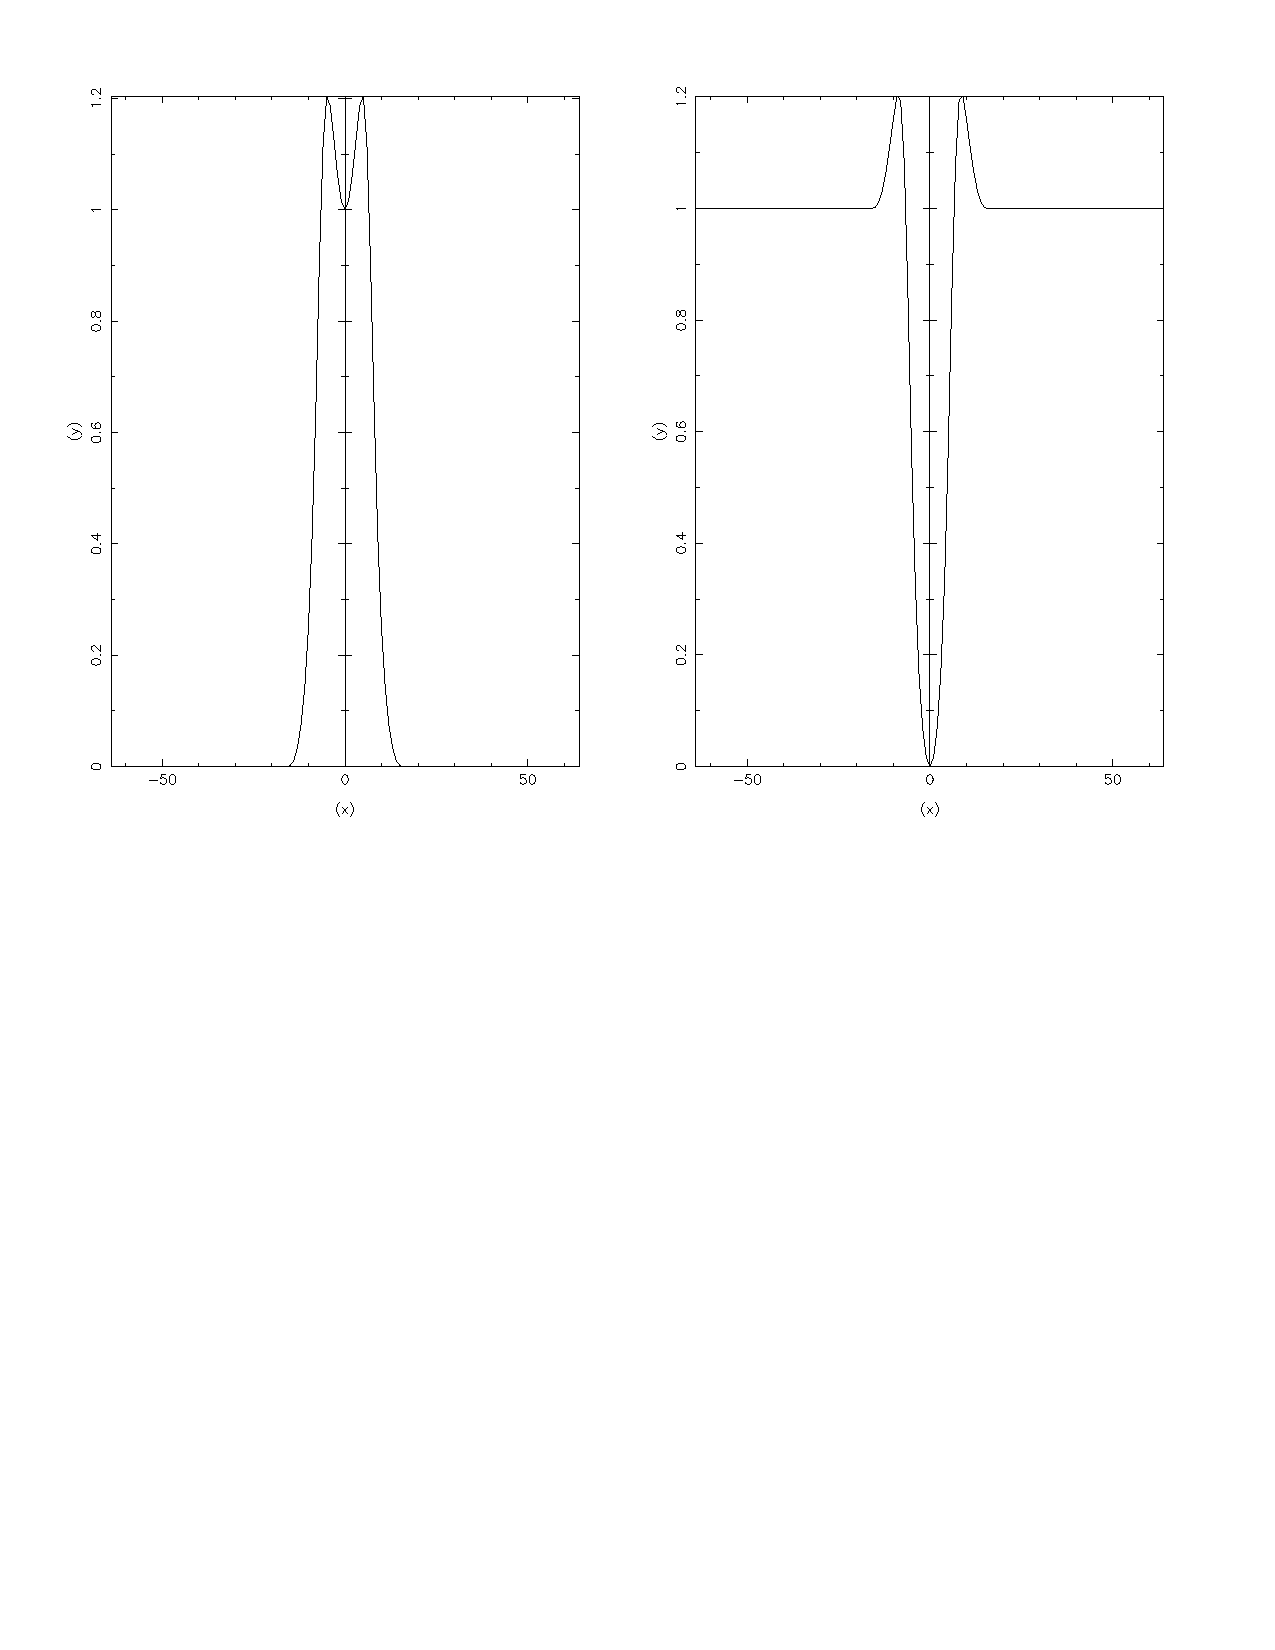
\includegraphics[width=14.5cm,height=5cm]{ch1_diff_uv_ht_gt.pdf}
}}}
\caption{On the left, the filter $\hat{\tilde{h}}$, and on the right the 
filter $\hat{\tilde{g}}$.}
\label{fig_diff_uv_ht_gt}
\end{figure}

But since the transform is redundant there is actually no unique way to reconstruct an image
from its coefficients (the filterbank design framework of Section~\ref{design_no_fb}). Indeed, using the relations:
\begin{eqnarray}
\begin{split}
\hat c_{j+1}[l,m] = \widehat H_{j} [l,m]  \hat c_{j} [l,m] \\
\hat w_{j+1}[l,m] = \widehat G_{j} [l,m] \hat c_{j} [l,m] 
\end{split}
\end{eqnarray}
a least-squares estimate of $c_j$ from $c_{j+1}$ and $w_{j+1}$ gives:
\begin{eqnarray}
\hat{c}_{j}   = \hat{c}_{j+1}  {\widehat {\tilde H}}_{j}   + \hat{w}_{j+1}  {\widehat {\tilde G}}_{j} ~,
\end{eqnarray}
where the dual filters $\tilde h$ and $\tilde g$ satisfy:
\begin{eqnarray}
\label{eqnht} 
\begin{split}
{\widehat {\tilde H}}_j =  \sqrt{\frac{4\pi}{2l+1} } {\hat {\tilde h}}_j & = {\widehat H}_{j}^* /
\parenth{\big|{\widehat H}_{j}\big|^2 + \big|{\widehat G}_j\big|^2} \\
{\widehat {\tilde G}}_j =  \sqrt{\frac{4\pi}{2l+1} } {\hat {\tilde g}}_j & = {\widehat G}_{j}^* /
\parenth{\big|{\widehat H}_j\big|^2 + \big|{\widehat G}_j\big|^2} .
\end{split}
\end{eqnarray}
For the scaling function which is a B$_3$-spline function and a wavelet taken as the difference between two resolutions,
the corresponding conjugate low pass and high pass filters $\widehat {\tilde H}$ and $\widehat {\tilde G}$ are plotted in Fig.~\ref{fig_diff_uv_ht_gt}. 
The reconstruction algorithm is given in Algorithm~\ref{algo_iuwts}.

{\linespread{1}
\begin{algorithm}[h]
\caption{Inverse UWT on the sphere.}
\label{algo_iuwts}
\noindent{\bf Task:} Reconstruct an image from its UWTS coefficients.\\
\noindent{\bf Parameters:} UWTS coefficients ${\cal W}=\{w_1, w_2, \dots, w_{J}, c_{J}\}$.\\
\noindent{\bf Initialization:}
\begin{itemize}
\item Compute the B$_3$-spline scaling function and derive $\hat{\psi}$, $\widehat{H}$, $\widehat{G}$, $\widehat{\tilde H}$ and $\widehat{\tilde G}$ numerically.
\item Compute the spherical harmonics transform of $c_J$ to get ${\hat c}_J$.
\end{itemize}
\For{$j=J-1$ to $0$, with step $=-1$} {
\begin{enumerate}[1.]
\item Compute the spherical harmonics transform of the wavelet coefficients $w_{j+1}$ to get $\hat{w}_{j+1}$.
\item Multiply $\hat{c}_{j+1}$ by ${\widehat {\tilde H}}_{j}$.
\item Multiply $\hat{w}_{j+1}$ by ${\widehat {\tilde G}}_{j}$.
\item Get the spherical harmonics of $\hat{c}_j=\hat{c}_{j+1}+\hat{w}_{j+1}$.
\end{enumerate}
}
Compute The inverse Spherical Harmonics transform of $\hat c_0$.\\
\noindent{\bf Output:} $c_0$ is the inverse UWT on the sphere.
\end{algorithm}

\begin{figure}[htb]
\centerline{
\hbox{
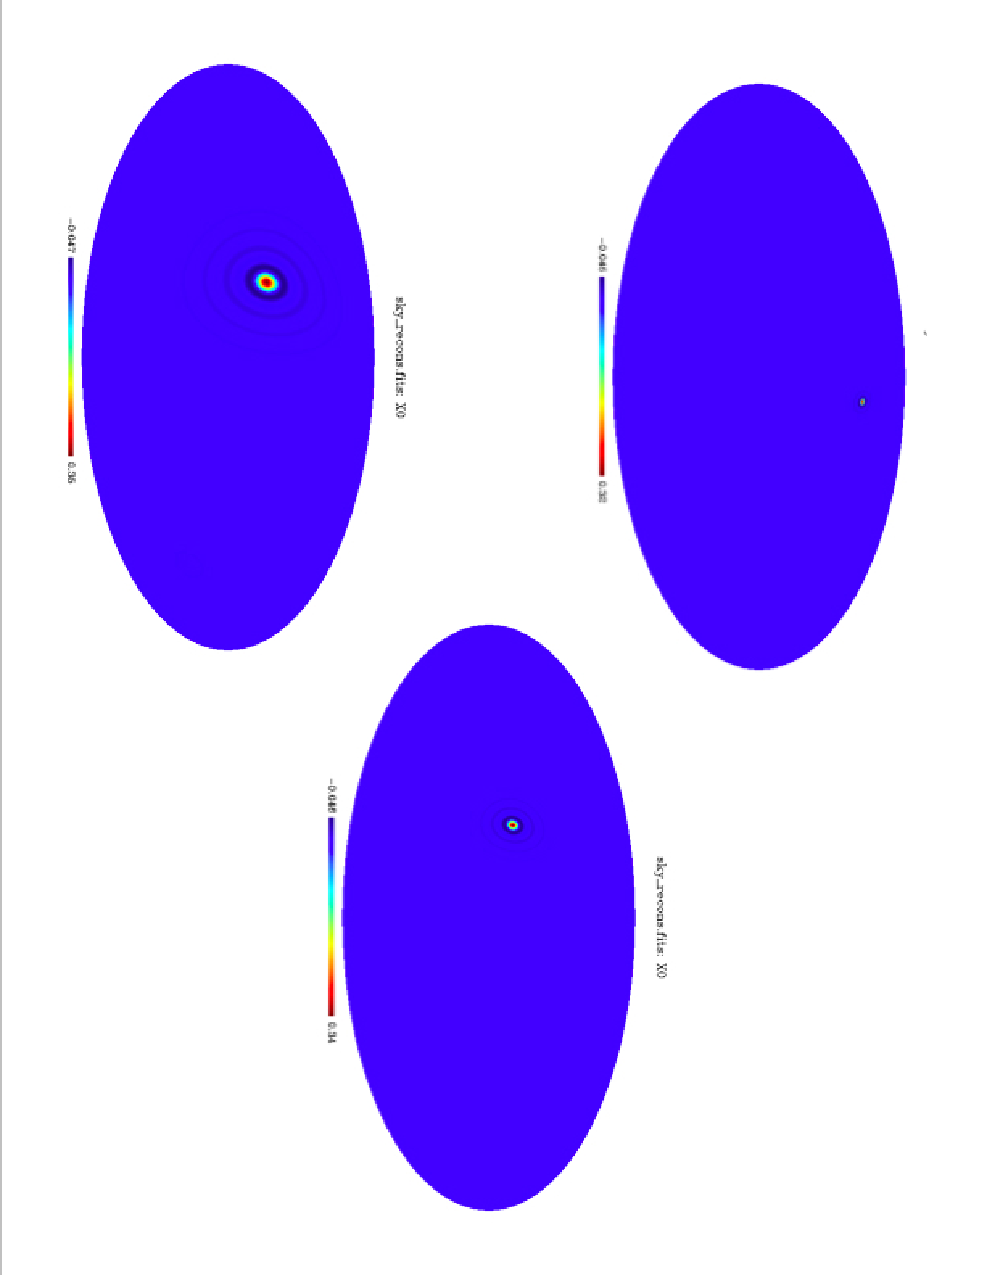
\includegraphics[width = 10cm,angle = 90]{fig_backwt_sphere.pdf}
}}
\caption{Reconstruction from a single wavelet coefficient at different scales. Each map is obtained by setting all wavelet coefficients to zero but one, and by applying an inverse UWTS. Depending on the position and scale of the non-zero coefficient, the reconstructed map shows an isotropic feature 
at different scales and positions.}
\label{Figure:back_wt}
\end{figure}
}
Fig.~\ref{Figure:back_wt} shows the reconstruction by setting all wavelet coefficients but one at different scales
and positions. Depending on the position and scale of the non-zero coefficient, the reconstructed map shows an isotropic feature 
at different scales and positions.
 

%-------------------------

\subsection{Isotropic Pyramidal Wavelet Transform on the Sphere}
\index{wavelet!pyramidal transform}
\index{sphere!pyramidal wavelet}

\subsubsection{Forward Transform}
In the previous algorithm, no down-sampling is
performed and each scale of the wavelet decomposition has the same number of pixels 
as the original data set. Therefore the number of pixels in the
decomposition is equal to the number of pixels in the data multiplied by the number of scales.
For some applications, we may prefer to introduce a decimation
in the decomposition so as to reduce the required memory size and the computation time.
This can be done easily by using a specific property of the chosen scaling function.
Indeed, since we are considering here a scaling function with an initial cut-off $l_c$ in spherical harmonic multipole number $l$, and since the actual cut-off is reduced by a factor of two at each step, the number 
of significant spherical harmonics coefficients is then reduced by a factor of four after each convolution with the low pass filter
$h$. Therefore, we need less pixels in the direct space when we compute the inverse 
spherical harmonics transform.  Using the HEALPix pixelization scheme \citep{pixel:healpix},  
this can be done easily by dividing by 2 the 
$N_{\mathrm{side}}$ parameter when calling the inverse spherical harmonics transform routine.
The pyramidal wavelet transform on the sphere algorithm is given in Algorithm~\ref{algo_pwts}.

{\linespread{1}
\begin{algorithm}[h]
\caption{Pyramidal wavelet transform on the sphere.}
\label{algo_pwts}
\noindent{\bf Task:} Compute the pyramidal WT on the sphere of a discrete image $X$.\\
\noindent{\bf Parameters:} Data $X$ and number of of wavelet scales $J$.\\
\noindent{\bf Initialization:} 
\begin{itemize}
\item $c_0=X$.
\item Compute the B$_3$-spline scaling function and derive $\hat{\psi}$, $\widehat{H}$ and $\widehat{G}$ numerically.
\item Compute the corresponding spherical harmonics transform of $c_0$.
\end{itemize}
\For{$j=0$ to $J-1$} {
\begin{enumerate}[1.]
\item Compute the spherical harmonics transform of the scaling coefficients:  $\hat{c}_{j+1}=\hat{c}_j\widehat{H}_{j}$.
\item Compute the inverse spherical harmonics transform of $\hat{c}_{j+1}$ to get $c_{j+1}$.
\item Down-sample $c_{j+1}$, since its support in the spherical harmonic domain has been divided by two.
\item Compute the spherical harmonics transform of the wavelet coefficients:  $\hat{w}_{j+1}=\hat{c}_j\widehat{G}_{j}$.
\item Compute the inverse spherical harmonics transform of $\hat{w}_{j+1}$ to get $w_{j+1}$.
\end{enumerate}
}
\noindent{\bf Output:} ${\cal W}=\{w_1, w_2, \dots, w_{J}, c_{J}\}$ the Pyramidal WT on sphere of $X$.
\end{algorithm}
}

\begin{figure}[htb]
\vbox{
\centerline{
\hbox{
 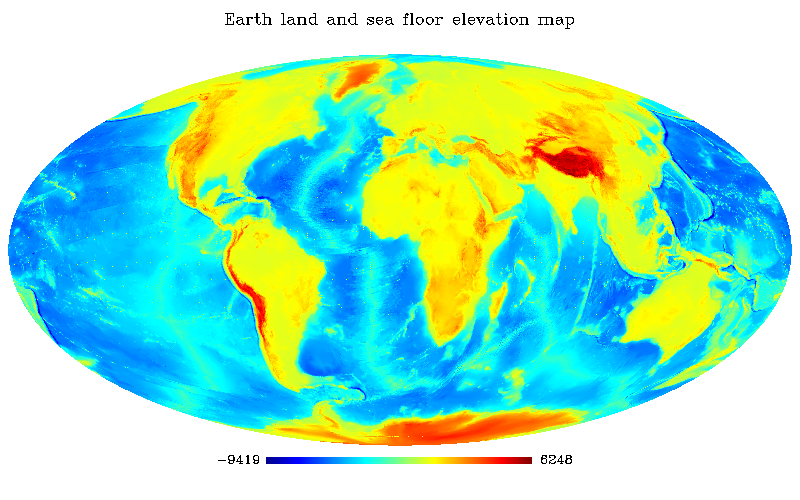
\includegraphics[width=6.5cm,height=3.9cm]{fig_earth_elevation.png}
 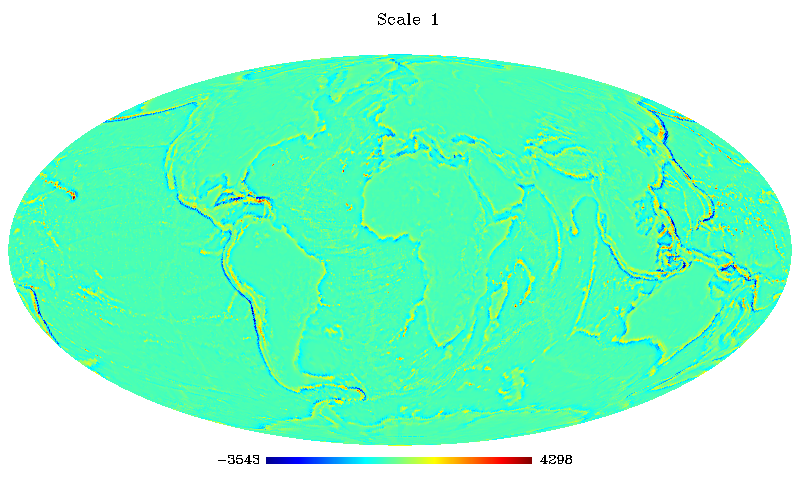
\includegraphics[width=6.5cm,height=3.9cm]{fig_earth_scale_1.png}
}}
\centerline{
\hbox{
 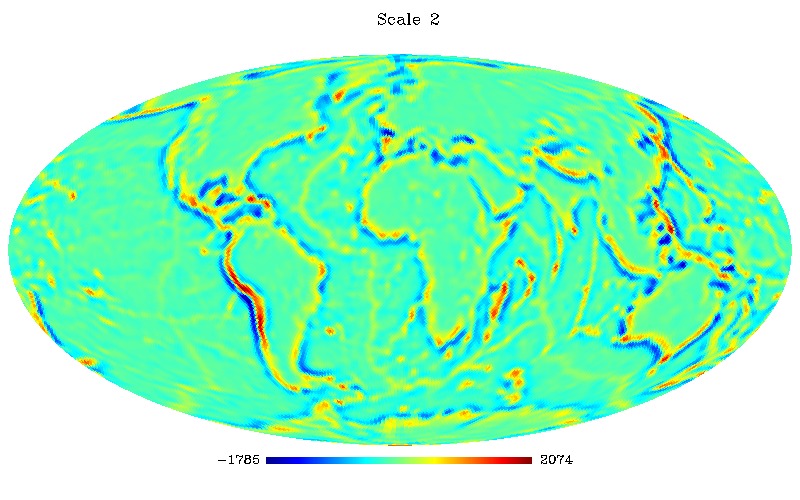
\includegraphics[width=6.5cm,height=3.9cm]{fig_earth_scale_2.png}
 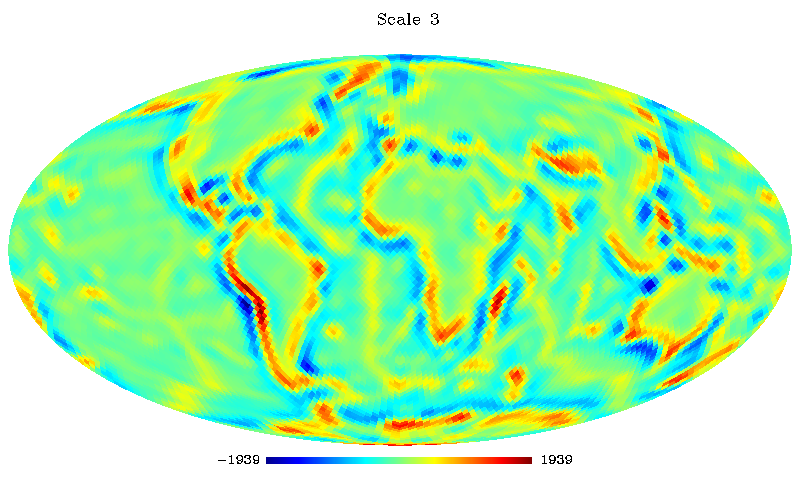
\includegraphics[width=6.5cm,height=3.9cm]{fig_earth_scale_3.png}
}}
\centerline{
\hbox{
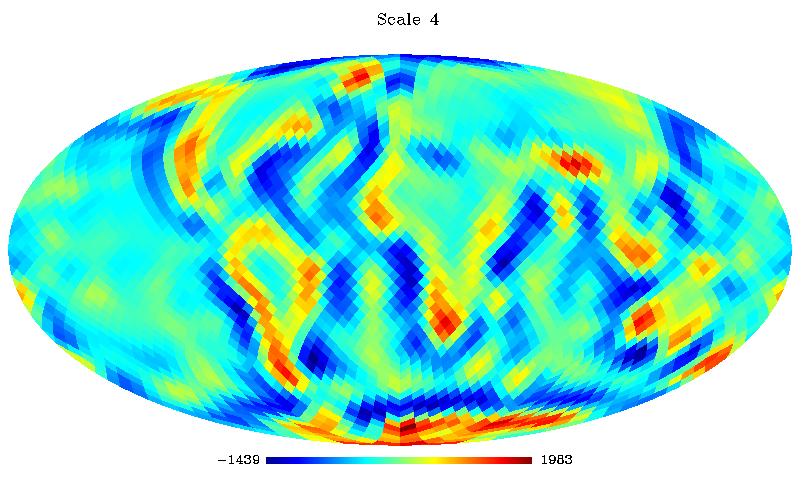
\includegraphics[width=6.5cm,height=3.9cm]{fig_earth_scale_4.png}
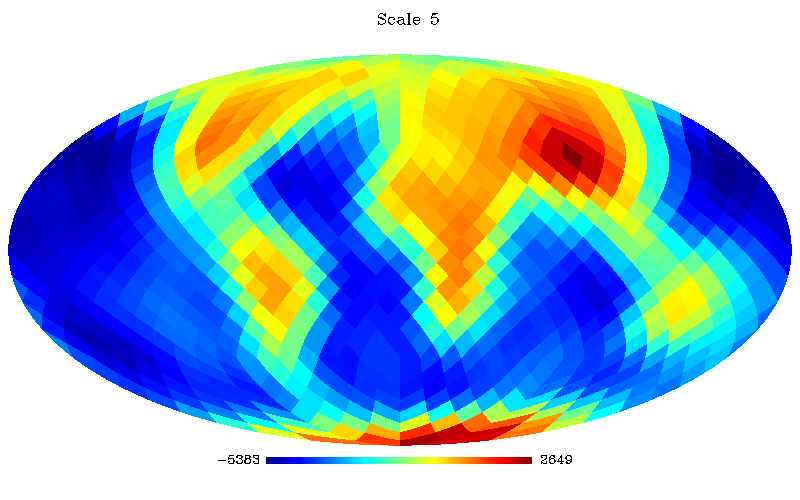
\includegraphics[width=6.5cm,height=3.9cm]{fig_earth_scale_5.png}
}}
}
\caption{Pyramidal wavelet transform on the sphere.}.
\label{Figure:PWTS}
\end{figure}

Fig.~\ref{Figure:PWTS} shows an Earth image and its pyramidal wavelet transform (PWTS) using five scales.
As the scale number increases (i.e.\ the resolution decreases), the pixel size becomes larger. The data are  land and sea-floor elevations  obtained from the ETOPO5 5-minute gridded elevation data set. A thorough explanation of the data set is provided at \texttt{www.ngdc.noaa.gov} \footnote{The ETOPO5 data are credited to ``Data Announcement 88-MGG-02, Digital relief of the Surface of the Earth. NOAA, National Geophysical Data Center, Boulder, Colorado, 1988''.   The HEALPix image is available at \texttt{http://astro.ic.ac.uk/$\sim$pdineen/earth/index.html\#earthmap}.}.


\newpage
\subsubsection{Inverse Transform}
 
This reconstruction is not as straightforward as in the undecimated case, since the different scales do not have the same resolution.
For each resolution level, we have to up-sample the scaling band before co-adding it to the wavelet coefficients. Algorithm \ref{algo_ipwts} describes this.
{\linespread{1}
\begin{algorithm}[h]
\caption{Inverse Pyramidal Wavelet Transform on the sphere.}
\label{algo_ipwts}
{\bf Task:} Reconstruct an image from its pyramidal WT on the sphere.\\
\noindent{\bf Parameters:} Pyramidal WT coefficients ${\cal W}=\{w_1, w_2, \dots, w_{J}, c_{J}\}$.\\
{\bf Initialization:}
\begin{itemize}
\item Compute the B$_3$-spline scaling function and derive $\hat{\psi}$, $\widehat{H}$, $\widehat{G}$, $\widehat{\tilde H}$ and $\widehat{\tilde G}$ numerically.
\item Compute the spherical harmonics transform of $c_J$ to get ${\hat c}_J$.
\end{itemize}
\For{$j=J-1$ to $0$} {
\begin{enumerate}[1.]
\item Upsample $c_{j+1}$ to the resolution of $c_j$.
\item Compute the spherical harmonics transform of the wavelet coefficients $w_{j+1}$ to get $\hat{w}_{j+1}$.
\item Multiply $\hat{c}_{j+1}$ by ${\widehat {\tilde H}}_{j}$.
\item Multiply $\hat{w}_{j+1}$ by ${\widehat {\tilde G}}_{j}$.
\item Get the spherical harmonics of $\hat{c}_j=\hat{c}_{j+1}+\hat{w}_{j+1}$.
\end{enumerate}
}
Compute The inverse spherical harmonics transform of $\hat c_0$.\\
\noindent{\bf Output:} $c_0$ is the inverse pyramidal WT on the sphere.
\end{algorithm}
}
  
The wavelet transform on the sphere and its pyramidal version have both a reconstruction operator, so they are very well designed for any restoration application when the data contains isotropic features. In the following, we present other transforms on the sphere more adapted to the analysis of anisotropic features.
 
%===============================================================================


\section{Curvelet Transform on the Sphere }
\label{sect_cur}
%\subsection{Introduction}
\index{curvelet}
\index{curvelet!sphere}
\index{sphere!curvelet}

The 2D curvelet transform enables the directional analysis of an image in different scales (see Chapter~\ref{ch_mga}). 
The fundamental property of the curvelet transform is to 
analyze the data with functions of length about
 $2^{-j/2}$ for the $j$th subband $[2^j, 2^{j+1}]$ of the 
two-dimensional wavelet transform.   
Following the implementation of the first generation curvelet transform described in Section~\ref{subsubsec_curvG1}, the data first undergoes 
an Isotropic Undecimated Wavelet Transform (i.e.\ starlet transform). Each scale $j$ is then decomposed into smoothly overlapping blocks of
side-length $B_j$ pixels in such a way that the overlap between two
vertically adjacent blocks is a rectangular array of size $B_j \times B_j/2$.
Finally the ridgelet transform is applied on each individual block. Recall from Chapter~\ref{ch_mga} that the ridgelet transform
precisely amounts to applying a 1D wavelet transform to the
slices of the Radon transform. The first generation curvelet transform is also redundant, with a redundancy factor of $16J+1$ whenever $J$ scales
are employed. The curvelet transform was shown to sparsely represent anisotropic structures and smooth curves and edges of different lengths.

\subsection{Curvelets on the Sphere}
The curvelet transform on the sphere (CTS) can be similar to the 2D first generation digital curvelet transform,
but replacing the starlet transform by the isotropic UWTS previously 
described. The CTS algorithm is the following:
\begin{itemize}
\item Isotropic UWTS. 
\item Partitioning: Each scale is decomposed into blocks of an appropriate scale (of side-length $\sim2^{-s}$), using the HEALPix pixelization.
\item Ridgelet transform: Each block is analyzed with the discrete ridgelet transform.
\end{itemize}
We now describe these three steps.

%\begin{figure}
%\centering
%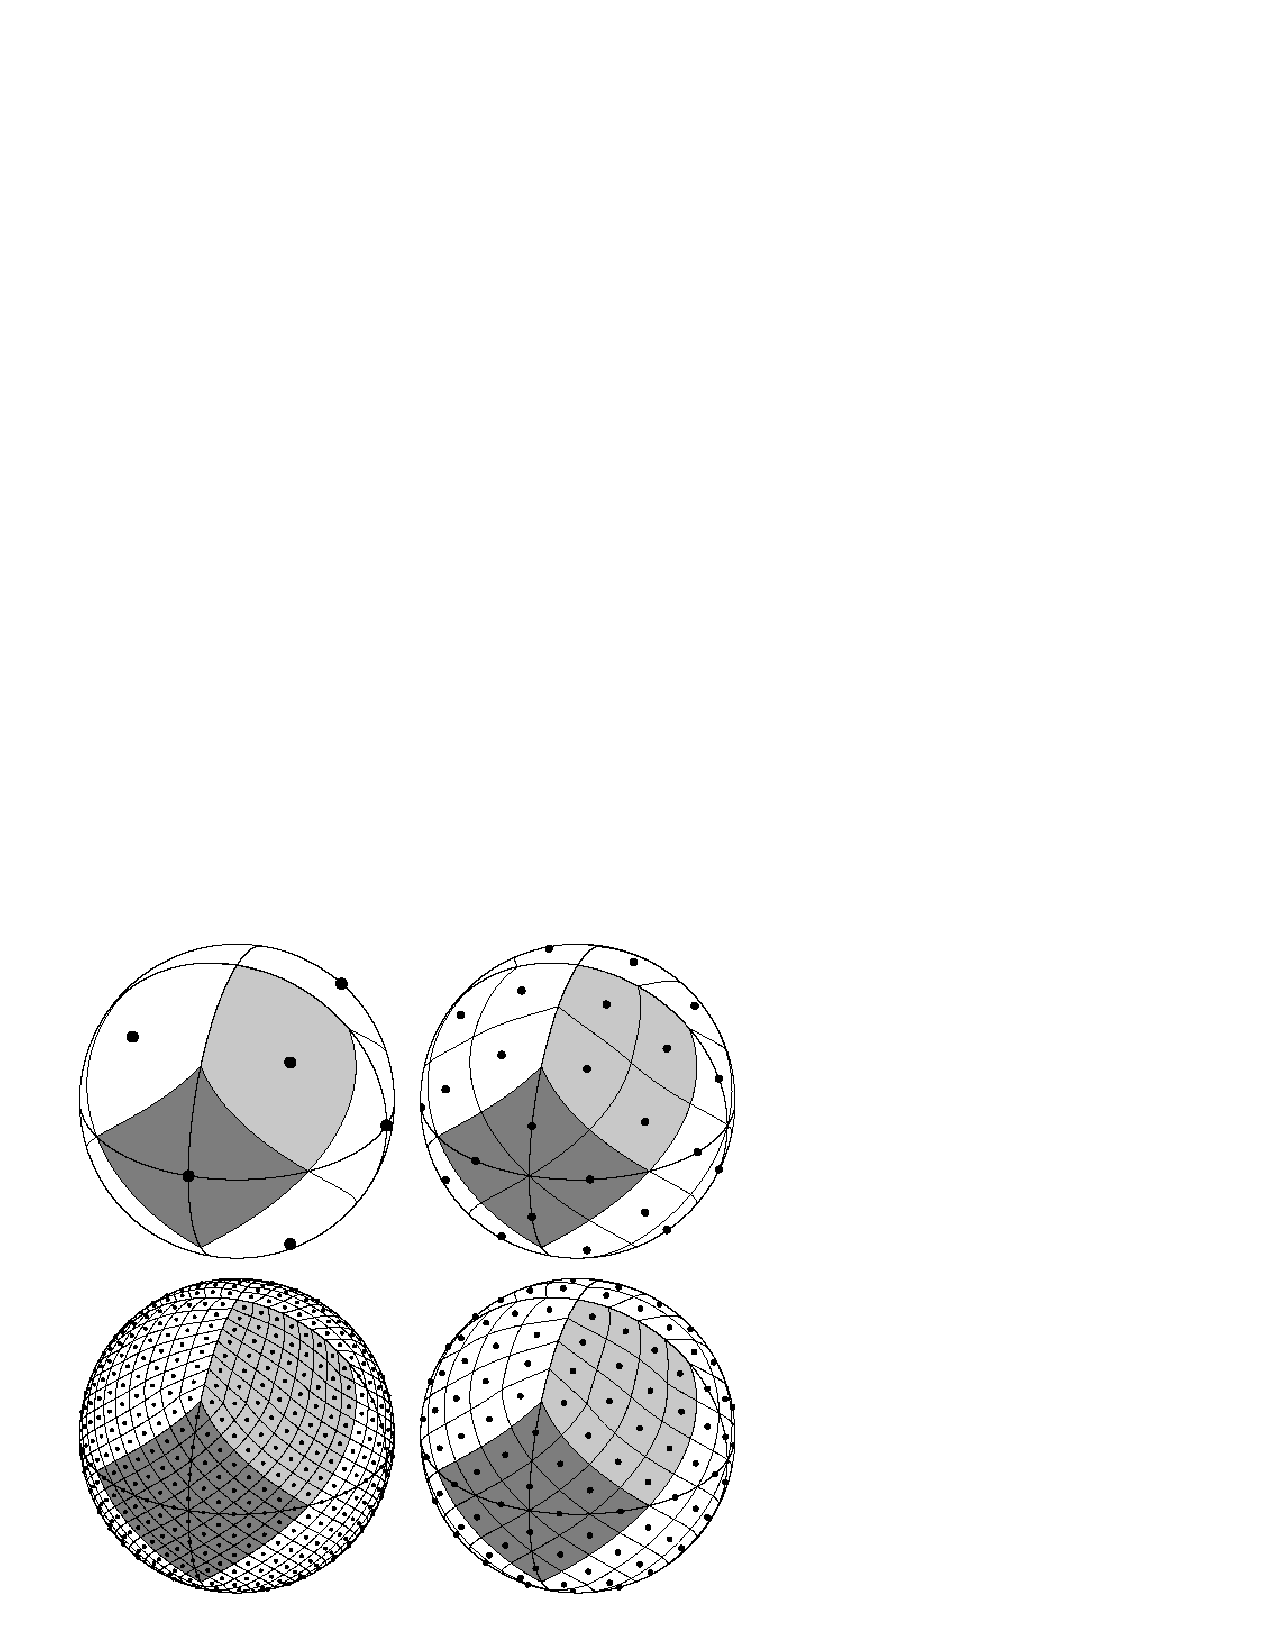
\includegraphics{pixelhealpix.pdf}
%\caption{The Healpix sampling grid.}
%\label{pixelhealpix}
%\end{figure}

\subsubsection{Partitioning Using the HEALPix Representation}
 
 \begin{figure}
\centerline{
\hbox{
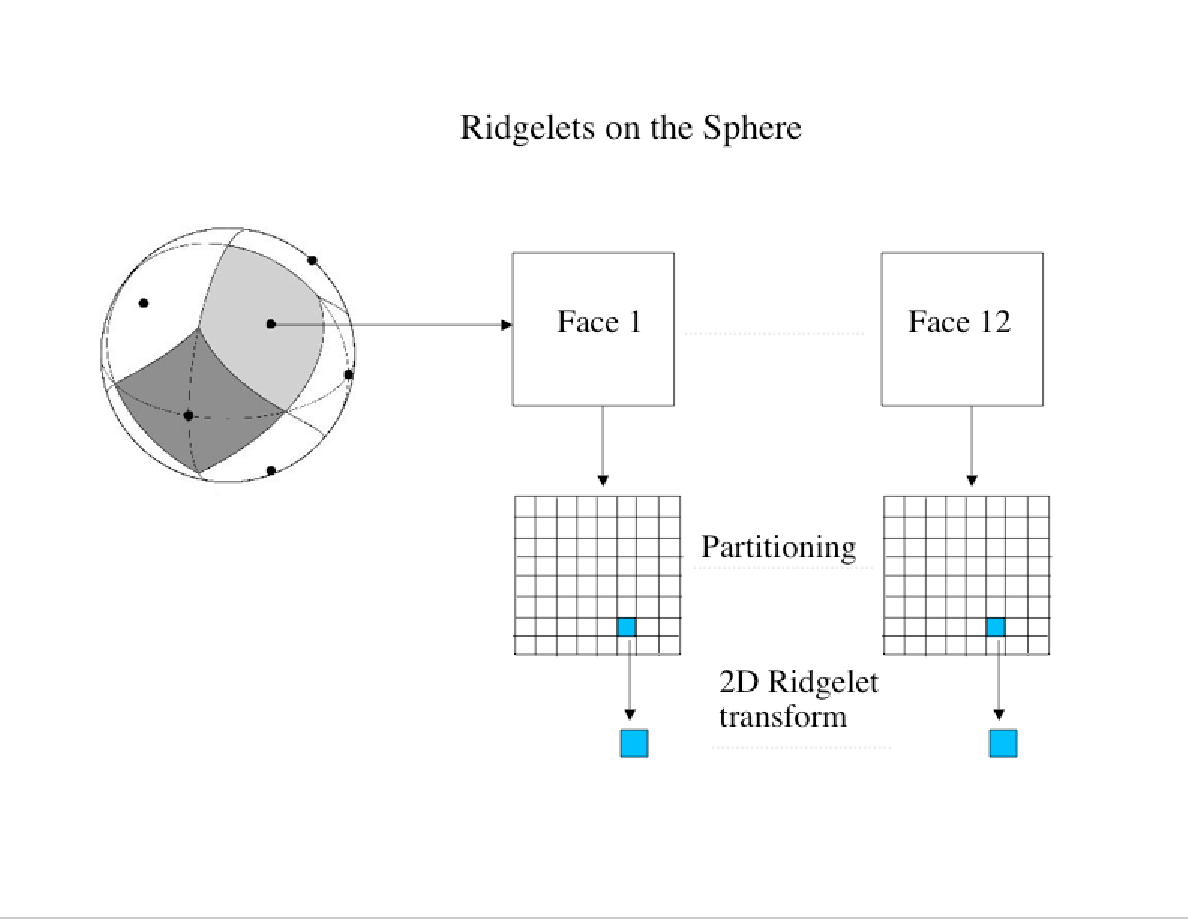
\includegraphics[width=12cm]{fig_flowgraph_ridgelet_sphere.pdf}
% \includegraphics[width=13.6cm,height=8cm]{fig_flowgraph_ridgelet_sphere.pdf}
}}
\caption{Flowgraph of the ridgelet transform on the sphere.}
\label{Figure:rid_sphere}
\end{figure}

The HEALPix representation is a curvilinear hierarchical partition of the sphere into quadrilateral pixels of exactly equal area but with varying shape. The base resolution divides the sphere into 12 quadrilateral faces of equal area placed on three rings around the poles and equator.  Each face is subsequently divided into $N_{\mathrm{side}}^{2}$ pixels following a quadrilateral multiscale  tree structure (see Fig.~\ref{pixelhealpix}).  The pixel centers are located on iso-latitude rings, and pixels from the same ring are equispaced in azimuth. This is critical for computational speed of all operations involving the evaluation of spherical harmonics transforms, including standard numerical analysis operations such as convolution, and  power spectrum estimation. 

An important geometrical feature of the HEALPix sampling grid is the hierarchical quadrilateral tree structure. This defines a  natural one-to-one mapping of the sphere sampled according to the HEALPix grid, into twelve  flat images, on all scales. It is then easy to partition a spherical map using HEALPix into quadrilateral blocks of a specified size. One first extracts  the twelve base-resolution faces, and each face is then decomposed into overlapping blocks of the specified size. This decomposition into blocks is an essential step of the traditional flat 2D curvelet transform. Based on the reversible warping of the sphere into a set of flat images made possible by the HEALPix sampling grid, the ridgelet and curvelet transforms can be extended to the sphere. 

With the decomposition into blocks described above, there is no overlap between neighboring blocks belonging to different base-resolution faces. This may result for instance in blocking effects in denoising experiments  via nonlinear filtering. It is possible to overcome this difficulty in some sense by working simultaneously  with various rotations of the data with respect to the sampling grid. This will average out undesirable effects at edges between base resolution faces. 

\newpage
\subsubsection{Ridgelet Transform}
\index{ridgelet}
\index{ridgelet!sphere}
\index{sphere!ridgelet}

Once the partitioning is performed, the standard 2D ridgelet transform described in Chapter~\ref{ch_mga} is applied  in each individual block. The ridgelet transform can be based on different implementations of the Radon transform: linogram, fast slant stack, see Chapter~\ref{ch_mga} for details. 
% \begin{enumerate}
% \item Compute the 2D Fourier transform.
% \item Extract lines going through the origin in the frequency plane.
% \item Compute  the 1D inverse Fourier transform of each line. We get the Radon transform.
% \item Compute the 1D wavelet transform of the lines of the Radon transform.
% \end{enumerate}
% The first three steps correspond to a Radon transform method called the 
% {\em linogram}.
% \index{linogram}
% Other implementations of the Radon transform,  such as the Slant Stack Radon Transform \citep{cur:donoho_02}, see Section \ref{sectfss}, 
% can be used as well, as long as they allow for an exact reconstruction.
\index{ridgelet transform!fast slant stack}   

Fig.~\ref{Figure:rid_sphere} shows the flowgraph of the ridgelet transform 
on the sphere and Fig.~\ref{Figure:back_rid} shows the reconstruction from a single ridgelet 
coefficient at different scales and orientations.


\begin{figure}[htb]
\centerline{
\hbox{
\includegraphics[width=10cm]{fig_ridssr.pdf}
% \includegraphics[width=9.5cm,height=6cm]{fig_ridssr.pdf}
}}
\caption{Ridgelet atoms on the sphere obtained by reconstruction from a few ridgelet coefficient at different scales and orientations.}
\label{Figure:back_rid}
\end{figure}

\subsection{Curvelet Transform Algorithm}
The curvelet transform algorithm on the sphere is described in 
Algorithm \ref{algo_curts}.
{\linespread{1}
\begin{algorithm}[h]
\caption{Curvelet Transform on the sphere.}
\label{algo_curts}
{\bf Task:} Compute the curvelet transform on the sphere of a discrete image $X$.\\
{\bf Parameters:} Image $X$ and number of scales $J$.\\
{\bf Initialization:} 
\begin{itemize}
\item $B_1 = B_{\min}$.
\item Compute the isotropic UWTS of $X$ with $J$ scales, get $\{w_1,\dots,w_J,c_J\}$.
\end{itemize}
\For{$j=0$ to $J-2$} {
\begin{enumerate}[1.]
\item Partition the wavelet subband $w_j$ with a block size $B_j$.
\item Apply the digital ridgelet transform to each block; get the curvelet coefficients at scale $j$.
\end{enumerate}
\lIf{$j \mbox{ modulo } 2 = 1$} $B_{j+1} = 2 B_{j}$,  else $B_{j+1} = B_{j}$.
}
{\bf Output:} The curvelet transform on the sphere of $X$.
\end{algorithm}
}
 
The sidelength of the localizing windows is doubled {\em at every
other} dyadic subband, hence maintaining the fundamental property of
the curvelet transform which says that elements of length about
$2^{-j/2}$ serve for the analysis and synthesis of the $j$th subband
$[2^j, 2^{j+1}]$.  We used the default value $B_{\min} = 16$
pixels in our implementation.  Fig.~\ref{Figure:cur_sphere}
gives an overview of the organization of the algorithm.

\begin{figure}[htb]
\vbox{
\centerline{
\hbox{
% \includegraphics[width=9.cm,height=12cm]{fig_flowgraph_curvelet_sphere.pdf}
\includegraphics[width=13cm]{fig_flowgraph_curvelet_sphere.pdf}
}}}
\caption{Flowgraph of the curvelet transform on the sphere.}
\label{Figure:cur_sphere}
\end{figure}

\begin{figure}
\vbox{
\centerline{
\hbox{
% \includegraphics[width=9.cm,height=12cm]{fig_back_cur_sphere.pdf}
\includegraphics[angle=90,width=12cm]{fig_back_cur_sphere.pdf}
}}}
\caption{Reconstruction from a single curvelet coefficient at different scales and orientations.}
\label{Figure:back_cur}
\end{figure}
Fig.~\ref{Figure:back_cur} shows the backprojection of  curvelet coefficients at 
different scales and orientations.

\subsection{Pyramidal Curvelet Transform on the Sphere}
The CTS is very redundant, which may be a problem for handling huge data sets such as 
Planck data (see Section \ref{section:cmb} below). 
The redundancy can be reduced by substituting, in the 
curvelet transform algorithm, the pyramidal wavelet transform with the undecimated wavelet transform.
The second step which consists of applying the ridgelet transform on the wavelet scale is unchanged.
The pyramidal curvelet transform (PCTS) algorithm is summarized in Algorithm~\ref{algo_pcurts}.
\index{sphere!pyramidal curvelet}

{\linespread{1}
\begin{algorithm}[h]
\caption{Pyramidal Curvelet Transform on the sphere.}
\label{algo_pcurts}
{\bf Task:} Compute the pyramidal curvelet transform on the sphere of a discrete image $X$.\\
{\bf Parameters:} Image $X$ and number of scales $J$.\\
{\bf Initialization:} 
\begin{itemize}
\item $B_1 = B_{\min}$.
\item Compute the pyramidal wavelet transform of $X$ with $J$ scales, get $\{w_1,\dots,w_J,c_J\}$.
\end{itemize}
\For{$j=0$ to $J-2$} {
\begin{enumerate}[1.]
\item Partition the wavelet subband $w_j$ with a block size $B_j$.
\item Apply the digital ridgelet transform to each block; get the curvelet coefficients at scale $j$.
\end{enumerate}
\lIf{$j \mbox{ modulo } 2 = 1$} $B_{j+1} = 2 B_{j}$,  else $B_{j+1} = B_{j}$.
}
{\bf Output:} The pyramidal curvelet transform on the sphere of $X$.
\end{algorithm}
}

In the next section, it is shown how the pyramidal curvelet transform can be used for image filtering.


%=========================================


\section{Restoration and Decomposition on the Sphere}
\label{sect_exp}

\subsection{Denoising}
\begin{figure}[htb]
\vbox{
\centerline{
\hbox{
 \includegraphics[width=6.5cm,height=3.9cm]{fig_sync.png}
 \includegraphics[width=6.5cm,height=3.9cm]{fig_sync_noise5.png}
}}
\centerline{
\hbox{
 \includegraphics[width=6.5cm,height=3.9cm]{fig_sync_wtfilter5.png}
 \includegraphics[width=6.5cm,height=3.9cm]{fig_sync_resi_wtfilter5.png}
}}
\centerline{
\hbox{
\includegraphics[width=6.5cm,height=3.9cm]{fig_sync_curfilter5.png}
\includegraphics[width=6.5cm,height=3.9cm]{fig_sync_resi_curfilter5.png}
}}
}
 \caption{Denoising. Upper left and right: simulated 
synchrotron image and same image with
additive Gaussian noise (i.e.\ simulated data).  Middle: undecimated 
wavelet filtering and residual.
Bottom: pyramidal curvelet filtering  and residual.}
\label{Figure:sync_filter}
\index{data!synchrotron}
\end{figure}


Wavelets and curvelets have been used successfully for image denoising via nonlinear filtering or thresholding methods as extensively studied in Chapter~\ref{chap:denoise}. In the results of Fig.~\ref{Figure:sync_filter}, denoising by hard thresholding the wavelet and curvelet coefficients on the sphere was used. The threshold was set to $4 \times $ the standard deviation of the noise at each subband.

% Hard thresholding, for instance, consists of setting all insignificant coefficients i.e.\ coefficients with an absolute value below a given threshold)
% to zero. In practice, we need to estimate the noise standard deviation $\sigma_j$ in each band $j$
% and a wavelet (or curvelet) coefficient $w_j$ is significant if $\abs{w_j} > \tau \sigma_j$,
% where $\tau$ is a user-defined parameter, typically chosen between 3 and 5. 
% The $\sigma_j$ estimation in band $j$ can be derived from simulations \citep{starck:book06}. 
% Denoting $\bf Y$ the noisy data and $\HT$ the thresholding operator, the filtered data $\bf X$ are obtained by:
% \begin{eqnarray}
%  {\bf X} =    {\W}   \HT_{\bf \lambda} ( {\W}^\Tr  {\bf Y} )
% \end{eqnarray}
% where ${\W}^\Tr$ is the wavelet (respectively, curvelet) 
% transform  and ${\W} $ is 
% the wavelet (resp.\ curvelet) reconstruction  (more details can be found in Chapter~\ref{chap:denoise}).
% $\bf \lambda$ is a vector which has the size of the number of bands in the used wavelet (respectively, curvelet) transform.
% The thresholding is applied to all coefficients in band $j$ with the threshold ${\bf \lambda}[j] = \tau \sigma_j$.

Fig.~\ref{Figure:sync_filter} describes the setting and the results of a simulated denoising experiment: upper left, the original simulated map of the  astrophysical synchrotron emission; upper right, the same image plus additive Gaussian noise ($\sigma=5$). Since the synchrotron image has a standard deviation (after renormalization) equal to $16.26$, the SNR is around  $3.25$.  The middle panels in this figure show the UWTS denoised image and the residuals.  The bottom panels show the pyramidal curvelet transform filtered image and the residuals. On such data, exhibiting very anisotropic features, the curvelets produce better results than wavelets.
  
\begin{figure}[htb]
\vbox{
\centerline{
\hbox{
 \includegraphics[width=8cm]{fig_sync_cbfilter5.png}
 }}
 \centerline{
 \hbox{
 \includegraphics[width=8cm]{fig_sync_resi_cbfilter5.png}
}}}
 \caption{Combined denoising (using both wavelets and curvelets) and residuals.}
\label{Figure:sync_cbf_filter}
\index{data!synchrotron}
\end{figure}

 \begin{table}[htb]
\baselineskip=0.4cm
\begin{center}
\begin{tabular}{lcccc} \hline \hline
Method                          &  Error standard deviation       \\ \hline \hline
Noisy map                       & 5    8  \\
Wavelet                         & 1.25     \\
Curvelet                        & 1.07   \\
CFA                             & 0.86  \\ \hline
\hline
\end{tabular}
\caption{Error standard deviations  after denoising the synchrotron noisy map (additive white Gaussian noise, $\sigma = 5$) by the wavelet, the curvelet and the combined denoising algorithm.  See Section~\ref{sect_cfm} for a description of the latter.}
\label{comptab_sync}
\end{center}
\end{table}


The residuals after wavelet and curvelet based denoising presented in Fig.~\ref{Figure:sync_filter} show different structures. As expected, elongated features are better restored using the curvelet transform, while isotropic structures are better denoised using the wavelet transform. The combined denoising algorithm introduced in Section~\ref{sect_cfm} can obviously also be applied on the sphere, in order to benefit from the advantages of both transforms. This iterative method detects the significant coefficients in both the wavelet domain and the curvelet domain and guarantees  that the reconstructed map will take into account any pattern which is detected as significant by either of the transforms. 

The results are reported in Table~\ref{comptab_sync}. The residual is much better when the combined denoising is applied, and no feature can be detected any more by eye in the residual (see Fig.~\ref{Figure:sync_cbf_filter}). This was not the case for either the wavelet or the curvelet based denoising alone.


% ==>  Err WT =       1.25165,  Err Cur  =       1.07169,  Err Combined =      0.857861



\subsection{Morphological Component Analysis}
\label{sect_mca}

% For a given spherical map ${\bf Y}$ modeled as a linear combination of 
% $K$ spherical maps $x_k$, $  {\bf Y} = \sum_{k=1}^K x_k$, having different 
% morphologies, 
% MCA assumes that a dictionary of bases $\{ \W_1,\cdots,\W_K \}$ exists such that, 
% for each $ ~ k$, $ x_k$ is sparse in $ ~ \W_k$ while its representation in the other $ ~ \W_{k'}$ ($ ~ k' \ne k$) is not sparse: 
% $ ~ \forall k' \neq k, ||\W_k^\Tr x_k||_0 < ||\W_{k'}^\Tr x_k||_0$, where $||x||_0$ denotes the $\ell_0$ pseudo-norm of the vector $x$.
% %  (\textit{i.e.}  the number of non-zero coefficients of $x$)
% The problem is to separate the mixture $\bf Y$ into its constitutive morphological components $ (x_k)_{k=1,\cdots,K}$ relying on the 
% discriminating power of the different dictionaries $\W_k$.  As described in Section~\ref{mca_method}, this can be done by minimizing
% \begin{equation}
% \label{eq:l1prob_sphere}
% \min_{x_1,\ldots,x_K}  \sum_{k=1}^K  \|  \W_k^\Tr  x_k \|_1   \mbox{ s.t. } \|  {\bf Y}  - \sum_{k=1}^K   x_k   \|_2 \leq \sigma
% \end{equation}
% where $\sigma$ is the noise standard deviation in the noisy case. 

The Morphological Component Analysis (MCA) Algorithm~\ref{algo:mca} (see Section~\ref{sec:mca}) was applied to a decomposition problem of an image on the sphere, using the transforms developed above.

The spherical maps shown in Fig.~\ref{Figure:mcatoy} illustrate a simple numerical experiment. We applied the MCA decomposition algorithm on the sphere, to synthetic data resulting from the linear mixture of components that were respectively sparse in the spherical harmonics and the isotropic wavelet representations. The method was able to separate the data back into its original constituents.  
 
\index{MCA}
\index{MCA!sphere}

\begin{figure}
\vbox{
\centerline{
\hbox{
% \includegraphics[width=6.5cm,height=4cm]{test_gauss_alm_bw.pdf}
\includegraphics[angle=90,width=6cm]{test_gauss_alm_bw.pdf}
}}
\centerline{
\hbox{
% \includegraphics[width=6.5cm,height=4cm]{test_gauss_alm_mca_alm_bw.pdf}
% \includegraphics[width=6.5cm,height=4cm]{test_gauss_alm_mca_wt_bw.pdf}
\includegraphics[angle=90,width=6cm]{test_gauss_alm_mca_alm_bw.pdf}
\includegraphics[angle=90,width=6cm]{test_gauss_alm_mca_wt.pdf}
}}
}
\caption{ Simple toy experiment with MCA on the sphere. 
The top map shows a linear combination of a spherical harmonic function 
and a localized Gaussian-like function on the sphere. The bottom maps 
show the resulting separated components that were obtained using the 
proposed Morphological Component Analysis on the sphere.}
\label{Figure:mcatoy}
\end{figure}

%---------------------------------------------------------------------------------------------------------------------------------------

\subsection{Inpainting}
\label{sect_mrs_inpaint}

\index{inpainting}
\index{inpainting!sphere}


%  Inpainting can also be done on the sphere. Consider a discrete spherical data map $\bf Y$ 
%  and the missing data mask ${ \bf M}_j$  
% (the main diagonal of ${\bf M}$ encodes the pixel status, namely $1$ for an existing
% pixel and $0$ for a missing one see, see Section~\ref{par:mcainpaint} for more details).
%  %  a boolean map $M$ such that ones in $M$ indicate that the corresponding pixels in $Y$ are valid data while zeros indicate invalid data. 
%  
% The objective function of MCA, 
% equation~\eqref{eq:l1prob_sphere}, can be modified as follows: 
% \begin{equation}
% \label{inp:model}
% \min_{x_1,\ldots,x_K}  \sum_{k=1}^K  \|  \W_k^\Tr  x_k \|_1   \mbox{ s.t. }  {\bf Y}   =  {\bf M}   \sum_{k=1}^K   x_k
% \end{equation}
% Thus we are preventing the sparse model under construction from attempting to fit the invalid data. 
% Other constraints can be easily imposed on the interpolated sparse components. 

The inpainting algorithms described in Section~\ref{sect_inpainting} can also be applied on the sphere. In Section~\ref{sect_inpainting}, a total variation penalty is shown to enhance the recovery of piecewise smooth components. Asking for regularity across the gaps of some localized statistics (e.g.\ enforcing the empirical variance of a given inpainted sparse component to be nearly equal outside and inside the masked areas) yields other possible constraints. In practice, because of the lack of accuracy of some digital transformations, additional constraints in the spherical topology can be used which may be relaxed close to convergence. These constraints were also found useful in some cases to stabilize the described iterative algorithms. 

A simple numerical experiment is shown in Fig.~\ref{Figure:mcaearth}. 
Starting with a full satellite view of the Earth\footnote{Available from: http://www.nasa.gov/vision/earth/features/bmng\_gallery\_4.html}, 
an incomplete spherical map was obtained by randomly masking some of the pixels. In fact, as much as sixty percent of the pixels were masked. Using both the spherical harmonics transform and the curvelet transform on the sphere within the proposed MCA inpainting algorithm, it is possible to fill in the missing pixels in a visually undetectable way. 

\begin{figure}[htb]
\vbox{
\centerline{
\hbox{
\includegraphics[angle=90,width=8cm]{earth_ori.pdf}
}}
\centerline{
\hbox{
\includegraphics[angle=90,width=8cm]{earth_mask.pdf}
}}
\centerline{
\hbox{
\includegraphics[angle=90,width=8cm]{earth_recons.pdf}
}}
}
 \caption{ Application of the proposed MCA-inpainting algorithm on the sphere. Top: original satellite view of the Earth.  
Middle: incomplete map retaining 40 percent of the original pixels. 
Bottom: inpainted map.}
\label{Figure:mcaearth}
\index{data!Earth}
\end{figure}

%=========================================================================

\section{Applications}
\subsection{Application in Fusion Physics}
\label{section:bedros}

\index{inertial confinement fusion}
\index{ICF}
\index{fusion physics}
In Inertial Confinement Fusion (ICF) a spherical shell is irradiated by laser energy directly or after the 
laser energy has been converted to soft X-rays~\citep{bedros:atzeni}. Either way, the aim is to implode the capsule which contains a shell of nuclear fusion fuel (deuterium and tritium) ready to ignite if, after it has been imploded, its density is high enough and a hot spot in its center becomes hot enough to cause a propagating nuclear burn wave to travel through the rest of the fuel. This ultimate energy source will not work if, during the implosion, hydrodynamic instabilities develop which can break apart the shell before it assembles at the center and a hot spot forms~\citep{bedros:lindl}. Hydrodynamic instabilities such as Rayleigh-Taylor occur due to non-uniformities in the laser spatial profile or imperfections in the composition of multiple surfaces which make up the layers of thin material that surround the nuclear  fuel. Very small amplitude imperfections initially can result in the ultimate failure of the target due to the large compression ratios involved in ICF.


\begin{figure}
\centerline{
\hbox{
\includegraphics[angle=0,width=6cm]{bed_mca_orig_data.png}
\includegraphics[angle=0,width=6cm]{bed_mca_large_scale.png}
}
}
\caption{Left: Surface structures of ICF spherical shells measured on the nanometer scale are a superposition of global scale variations, isolated bumps and scratches as well as artifacts which look like interference patterns on intermediate scales. Right: Coarsest scale of the undecimated isotropic wavelet transform of the surface measurements of an ICF target.}
\label{bedros_mca_data}
\index{data!plasma confinement}
\end{figure}
\begin{figure}[htb]
\centerline{
\includegraphics[angle=0,width=6cm]{bed_mca_in_data.png}
\includegraphics[angle=0,width=6cm]{bed_mca_large_scale.png}
}
\centerline{
\includegraphics[angle=0,width=6cm]{bed_mca_out_dct.png}
\includegraphics[angle=0,width=6cm]{bed_mca_out_wt.png}
}
\caption{Top: Spherical map obtained by subtracting the coarse scale map on the right of Fig.~\ref{bedros_mca_data} from the initial map on the left of Fig.~\ref{bedros_mca_data}. Bottom: Component maps separated by the MCA method on the sphere: interference patterns and measurement artifacts were caught by the local cosine functions on the sphere (left) while  the isolated bumps were caught using the undecimated wavelet on the sphere (right). Adding back the coarse scale on the right of Fig.~\ref{bedros_mca_data} to the latter map results in a clean map of the surface structures of an ICF spherical shell with the interference patterns and artifacts removed.} 
\label{bedros_mca_result}
\index{data!plasma confinement}
\end{figure}

It is therefore extremely important to characterize the inner and outer surfaces of ICF shell targets so as to know whether they are worthy of consideration for ICF implosions. One day in a reactor setting tens of thousands of targets will have to be imploded daily so that checking each one is totally out of the question. Instead, very good target fabrication quality control processes have to be adopted so that confidence levels in proper performance will be high. A major step along this path to fusion energy then is to understand why imperfections occur and to correct the systematic elements and control the harm done by random sources.
%
Fine structures on the surfaces of spherical shells can be measured on the nanometer scale, among others,  by atomic force microscopy or phase shifting spherical diffractive optical interferometry. 

An example of such measurements is shown in Fig.~\ref{bedros_mca_data}. As can be seen from the figure, there appears to be a superposition of global scale variations, isolated bumps and scratches as well as artifacts which look like interference patterns on intermediate scales of localization. The latter must be isolated and eliminated from consideration when deciding the readiness of the target for implosion. 

We achieved morphological feature separation by first doing an isotropic wavelet transform on the spherical data and subtracting the coarsest scale information. MCA on the sphere was used on the rest of the image using the undecimated wavelet and the local cosine transforms on the sphere. The isolated bumps were thus identified and the artifacts caused by the measurement technique were removed easily. The resulting bumps, added to the coarsest scale, comprises the clean data with the interference patterns and artifacts removed as shown in Fig.~\ref{bedros_mca_result}. The spherical harmonic decomposition of the cleaned image gives rise to coefficients of various $\ell$ modes which will be amplified by the implosion process.

The implosion process can now be assessed correctly using numerical hydrodynamic simulation generated growth factors. If the bumps are clustered and not randomly distributed then systematic errors in the manufacturing process can be tracked down. 
%A code called MODEM has been put together to study such target surface data and extract the localized bump statistics including their correlations in height, size and relative location. 
For more details see~\citet{bedros:modem}.
 
 
\subsection{Application in Cosmology}
\label{section:cmb}

A major issue in modern cosmology is the measurement and the statistical characterization  (spatial power spectrum, Gaussianity)  of the slight fluctuations in the Cosmic Microwave Background radiation field. These are strongly related to  the cosmological scenarios describing the properties and evolution of our Universe. Some 370,000 years after the Big Bang, when the temperature of the Universe was around 3000~K, thermal energy was no longer sufficient to keep electrons and positively charged particles apart so they combined. Photons were then set free in a nearly transparent Universe. Since the Universe further expanded, these photons are now in the microwave range but they should still be distributed according to a black body emission law. Indeed, before recombination, the Universe was a highly homogeneous opaque plasma in near thermal equilibrium in which photons and charged particles were highly interacting.  Hence the slight fluctuations in matter density, from which such large scale structures as galaxies or clusters of galaxies have evolved, are also imprinted on the distribution of photons. 
\begin{figure}[htb]
\vbox{
\centerline{
\hbox{
\includegraphics[width = 6.cm]{ADAIV_poster_abrial_fig1}
\includegraphics[width = 6.cm]{ADAIV_poster_abrial_fig2}
}
}
}
\caption{Left: CMB data map provided by the WMAP team. Areas of significant foreground contamination in the galactic region and at the locations of strong radio point sources have been masked out. Right: Map obtained by applying the  MCA-inpainting algorithm on the sphere to the former incomplete WMAP CMB data map.}
\label{cmb_wmap_inpainting}
\index{data!CMB}
\end{figure}

\index{CMB}
\index{Cosmic Microwave Background}
The Cosmic Microwave Background (CMB) was first observed in 1965 by Penzias and Wilson confirming a prediction made by Gamow in the late 1940s. But it was not until the early 1990s that evidence for small fluctuations in the CMB sky could finally be found thanks to the observations made by COBE~\citep{gauss:smoot92}. This was confirmed by several subsequent observations and recently by NASA's Wilkinson Microwave Anisotropie Probe (WMAP) \footnote{The WMAP data and mask we used here are available online at http://map.gsfc.nasa.gov/}. Full-sky multi-spectral observations with unprecedented sensitivity and angular resolution are expected from ESA's Planck\footnote{http://astro.estec.esa.nl/Planck} mission, which was launched in 2009. The statistical analysis of this data set will help set tighter bounds on major cosmological parameters.

\begin{figure}[htb]
\vbox{
\centerline{
\hbox{
\includegraphics[width=5cm]{ADAIV_poster_abrial_fig6}
\includegraphics[width=5cm]{ADAIV_poster_abrial_fig7}
}
}
\centerline{
\hbox{
\includegraphics[width=5cm]{ADAIV_poster_abrial_fig8}
\includegraphics[width=5cm]{ADAIV_poster_abrial_fig9}
}
}
\centerline{
\hbox{
\includegraphics[width=5cm]{ADAIV_poster_abrial_fig10}
\includegraphics[width=5cm]{ADAIV_poster_abrial_fig11}
}
}
\centerline{
\hbox{
\includegraphics[width=5cm]{ADAIV_poster_abrial_fig12}
\includegraphics[width=5cm]{ADAIV_poster_abrial_fig13}
}
}
}
\caption{Top left: Masked area. From top to bottom and left to right: The seven wavelet scales of the inpainted map. From the visual point  of view, the initially masked area cannot be distinguished any more in the wavelet scales of the inpainted map.}
\label{cmb_scale_wmap_inpainting}
\end{figure}

A simple numerical experiment is shown in Fig.~\ref{cmb_wmap_inpainting}, starting with the full-sky CMB map provided by the WMAP team.
% and available at http://map.gsfc.nasa.gov/. 
This CMB map was partially masked to discard pixels where the level of  contamination by residual foregrounds is expected to be the highest. Applying the described inpainting algorithm, making use of the sparsity of the representation of CMB in the spherical harmonics domain, leads to the map shown on the right of Fig.~\ref{cmb_wmap_inpainting}: the stationarity of the CMB field appears to have been restored and the masked region is completely undetectable to the eye.  Fig.~\ref{cmb_scale_wmap_inpainting} shows the wavelet decomposition of the inpainted map allowing for further visual positive assessment of the quality of the proposed method as again the masked regions are undetectable at all scales. It was shown in \citet{inpainting:abrial06,starck:abrial08} that inpainting the CMB map is an interesting approach for analyzing it, especially for non-Gaussianity studies and power spectrum estimation.


\newpage
\section{Guided Numerical Experiments}
\subsection{MR/S Toolbox}
The guided numerical experiments of this chapter are conducted using IDL with HEALPix and MR/S toolboxes. 

The IDL software  (\texttt{http://www.idl-envi.com}) is analogous to Matlab and is very widely used in astrophysics and in medical imaging.  
HEALPix is available at 
\texttt{http://sourceforge.net/projects/healpix}.
MR/S is a collection of IDL files that implements all the multiscale transforms described in 
this chapter, using HEALPix pixelization. The library is available via the book's web site: 

{\centerline{\texttt{http://www.SparseSignalRecipes.info}}}

% MR/S is available for download at:  \\
% {\centerline{\texttt{http://jstarck.free.fr/mrs.html}}}

\subsection{Undecimated Wavelet Transform on the Sphere}
The code to generate the undecimated wavelet transform of the Mars 
image of Fig.~\ref{Figure:UWTS} is as follows. 
\begin{verbatim}
; read the data 
m = mrs_read('mars_topo_mola_hpx_128.fits')

; compute the undecimated wavelet transform with 5 scales
mrs_wttrans, m, w,nbrscale=5

; Display and write the figures to the disk
tvs, m, tit='Mars topographic map', png='fig_mars.png'
tvs, w.coef[*,0], tit='Mars topographic map: scale 1', $
                   png='fig_mars_scale1.png' 
tvs, w.coef[*,1], tit='Mars topographic map: scale 2', $
                   png='fig_mars_scale2.png'
tvs, w.coef[*,2], tit='Mars topographic map: scale 3', $
                   png='fig_mars_scale3.png'
tvs, w.coef[*,3], tit='Mars topographic map: scale 4', $
                   png='fig_mars_scale4.png'
tvs, w.coef[*,4], tit='Mars topographic map: scale 5', $
                   png='fig_mars_scale5.png'
\end{verbatim}

\subsection{Pyramidal Wavelet Transform on the Sphere}
The code to generate the pyramidal wavelet transform of the Mars 
image of Fig.~\ref{Figure:PWTS} is as follows.  
\index{sphere!pyramidal wavelet}

\begin{verbatim}
; read the data 
e = mrs_read('earth_healpix_128.fits')

; compute the pyramidal wavelet transform with 5 scales
mrs_pwttrans, e, we, nbrscale=5

; Display and write the figures to the disk
mrs_wttv, we, write='fig_earth'
\end{verbatim}


\subsubsection{Denoising}
In the denoising experiment of Fig.~\ref {Figure:sync_filter} and Fig.~\ref{Figure:sync_cbf_filter}, 
we have added Gaussian noise to the astronomical simulated synchrotron emission map.
The code to generate the figures is as follows.
\begin{verbatim}
; read the image
s = rims('sync_res128.fits')

; add Gaussian noise
n = randomn(seed, N_ELEMENTS(s))
SigmaNoise = 5.
s1 = s + n* SigmaNoise
 
; Denoising using the undecimated WT on the sphere at 4sigma
Nsig = 4.
 mrs_wtfilter, s1, fwt4, nsigma= Nsig, nbrscale=5, SigmaNoise=SigmaNoise

; Denoising using the curvelet transform
mrs_curfilter, s1, fct4, nsigma= Nsig, nbrscale=5, SigmaNoise=SigmaNoise

; Denoising using the combined denoising
mrs_cbfilter, s1, fcb4, nsigma= Nsig, nbrscale=5, SigmaNoise=SigmaNoise

; Display and write the figure to the disk
tvs, s, /log, tit='Synchrotron emission', png='fig_sync.png'
tvs, s1 > 30, /log, tit='Synchrotron emission + noise', $
                   png='fig_sync_noise5.png'

tvs , fwt4 > 30, /log, title='Undecimated Wavelet Denoising (4sigma)', $
                   png='fig_sync_wtfilter5.png'
tvs , fct4 > 30, /log, title='Curvelet Denoising (4sigma)',  $
                   png='fig_sync_curfilter5.png'
tvs , fcb4 > 30, /log, title='Combined Filtering (4sigma)',  
                   png='fig_sync_cbfilter5.png'

tvs , s1- fwt4,   title='Residual undecimated Wavelet Denoising (4sigma)', $
                   png='fig_sync_resi_wtfilter5.png'
tvs , s1 - fct4,  title='Residual  curvelet Denoising (4sigma)',  $
                   png='fig_sync_resi_curfilter5.png'
tvs , s1  - fcb4,  title='Residual  combined Filtering (4sigma)',  $
                   png='fig_sync_resi_cbfilter5.png'

; Print the standard deviation (error) between the true image 
; and the denoised images
print, 'Err WT = ', sigma(s-fwt4) , ', Err Cur  = ', sigma(s-fct4),  ',  $
                  Err Comb = ', sigma(s-fcb4)

\end{verbatim}

We find the outcome here to be:

\begin{verbatim}
==>  Err WT = 1.25,  Err Cur  = 1.07,  Err Combined = 0.86
\end{verbatim}


\section{Summary}
In this chapter, multiscale transforms on the sphere were presented: the wavelet transform, the ridgelet transform and the curvelet transform. The described transforms have many desirable properties such as invertibility. With the wealth of these multiscale analysis tools and the associated discrete analysis and synthesis transforms on the sphere at hand, several problems with spherical data can be attacked effectively.  
Applications to denoising, image decomposition and inpainting on the sphere were given. Few applications to challenging data analysis problems in physics and astrophysics were reported. These tools are expected to be valuable in many other applications. To disseminate them, a toolbox implementing both the transforms and the denoising, separation and inpainting algorithms is freely available to interested users.
  

